% ============================================================
% BÖLÜM 4 - SAYISAL DENEYLER VE BULGULAR
% ============================================================
\chapter{SAYISAL DENEYLER VE BULGULAR}
\label{ch:bulgular}

\section{LES Referans Veri Setinin Üretimi}
\label{sec:les_referans}

INNATE modelinin doğrulanmasında \emph{referans gerçek} olarak benimsenmek üzere bağımsız bir LES çözücüsü uygulanmıştır. LES çözücüsü, Bölüm~\ref{ch:teorik}'te tanıtılan Smagorinsky alt-ızgara modelini ($C_{s}=0.17$), klasik dördüncü mertebe Runge--Kutta zaman ilerletmesini ve pseudo-spektral türev hesaplamalarını içerir. Boussinesq kaldırma kuvveti kaynaklı doğrusal kararsızlık modlarını bastırmak için Bölüm~\ref{sec:anisotropic_damping}'te tanımlanan anizotropik damping profili uygulanmıştır.

LES çözücüsünün ana özellikleri şu şekildedir:
\begin{itemize}
  \item Pseudo-spektral türev hesaplaması (3D anizotropik FFT, $2/3$ dealiasing kuralı),
  \item RK4 zaman entegrasyonu, adaptif zaman adımı (CFL $\leq 0.5$),
  \item Smagorinsky kapanışı: $\nu_{t} = (C_{s}\Delta)^{2}|S|$, türbülans Prandtl sayısı $\mathrm{Pr}_{t}=0.85$,
  \item Spektral Leray projeksiyonu ile diverjans-serbest garantisi,
  \item Boussinesq kaldırma kuvveti: $\mathrm{Ri}\,\theta\,\hat{\mathbf{e}}_{y}$,
  \item Kolmogorov forcing: $F_{x}(\mathbf{x}) = A\sin(k_{f}y)$, $k_{f}=4$, $A=0.005$,
  \item Anizotropik elevator-mode damping ($v$ ve $\theta$ üzerinde),
  \item Periyodik sınır koşulları (her üç yönde),
  \item Float32 hassasiyet (LES için yeterli).
\end{itemize}
Tek bir RK4 adımının özet kodu Kod~\ref{code:les_step}'de verilmiştir.

\begin{lstlisting}[caption={LES çözücüsü RK4 adımı (özet). Tam dosya: \texttt{les\_solver.py}.}, label={code:les_step}]
def rhs(self, u, v, w, theta, p):
    """LES sağ-tarafı: tüm fiziksel terimler."""
    # Adveksiyon (skew-symmetric, dealiased)
    adv_u, adv_v, adv_w = self.advection(u, v, w)
    th_adv = self.thermal_advection(u, v, w, theta)
    # Smagorinsky eddy viskozitesi
    S_mag = self.strain_rate_magnitude(u, v, w)
    nu_t = (self.Cs * self.Delta)**2 * S_mag
    kappa_t = nu_t / self.Pr_t
    # Difüzyon: (nu + nu_t) * lap u
    diff_u = (self.nu + nu_t) * self.laplacian(u)
    diff_v = (self.nu + nu_t) * self.laplacian(v)
    diff_w = (self.nu + nu_t) * self.laplacian(w)
    diff_theta = (self.kappa + kappa_t) * self.laplacian(theta)
    # Boussinesq + forcing + termal kaynak
    buoy_v = self.Ri * theta
    Fx = self.forcing_amplitude * torch.sin(self.k_f * self.y_grid)
    src_theta = v * self.dT / self.Ly      # baz gradyan kaynağı
    # Basınç gradyanı
    dp_dx, dp_dy, dp_dz = self.gradient(p)
    # Anizotropik damping (v + theta üstüne)
    damp_v     = -self.gamma_damp * v
    damp_theta = -self.gamma_damp * theta
    # Toplam RHS
    rhs_u = -adv_u + diff_u           - dp_dx + Fx
    rhs_v = -adv_v + diff_v + buoy_v  - dp_dy + damp_v
    rhs_w = -adv_w + diff_w           - dp_dz
    rhs_t = -th_adv + diff_theta + src_theta + damp_theta
    return rhs_u, rhs_v, rhs_w, rhs_t

def step_rk4(self, u, v, w, theta, p, dt):
    k1 = self.rhs(u, v, w, theta, p)
    k2 = self.rhs(*(x + 0.5*dt*k for x,k in zip((u,v,w,theta), k1)), p)
    k3 = self.rhs(*(x + 0.5*dt*k for x,k in zip((u,v,w,theta), k2)), p)
    k4 = self.rhs(*(x +     dt*k for x,k in zip((u,v,w,theta), k3)), p)
    u_new     = u     + dt/6 * (k1[0] + 2*k2[0] + 2*k3[0] + k4[0])
    v_new     = v     + dt/6 * (k1[1] + 2*k2[1] + 2*k3[1] + k4[1])
    w_new     = w     + dt/6 * (k1[2] + 2*k2[2] + 2*k3[2] + k4[2])
    theta_new = theta + dt/6 * (k1[3] + 2*k2[3] + 2*k3[3] + k4[3])
    # Spektral Leray projeksiyon: div-free garanti
    u_new, v_new, w_new, p_new = self.leray_projection(u_new, v_new, w_new)
    return u_new, v_new, w_new, theta_new, p_new
\end{lstlisting}

\subsection{Çalışma Noktasının Belirlenmesi}

LES çalışma noktasının belirlenmesi sürecinde sistematik bir tarama yapılmıştır. $\mathrm{Re}=5000$ ve $\mathrm{Ra}=10^{5}$ kombinasyonu test edildiğinde, Richardson sayısının $\mathrm{Ri}\approx 5.6\times 10^{-3}$ değerine ulaştığı ve buoyancy-driven elevator modlarının damping'e rağmen istatistiksel olarak doygunluğa erişemediği gözlenmiştir; bu rejim çalışmadan çıkarılmıştır. $\mathrm{Re}=7000$ ve $\mathrm{Re}=10\,000$ değerleri, daha düşük Richardson sayıları sayesinde kararlı ve tekrarlanabilir istatistikler ürettiği için final çalışma noktaları olarak benimsenmiştir.

\subsection{LES Sonuçları}

İki Reynolds sayısı için 60\,000 zaman adımı uzunluğunda LES simülasyonları yapılmış, son 10\,000 zaman adımı üzerinden istatistikler hesaplanmıştır. Sonuçlar Tablo~\ref{tab:les_summary}'de özetlenmiştir.

\begin{table}[H]
\centering
\caption{LES referans çözümlerinin istatistiksel özeti. Tüm değerler son 10\,000 zaman adımı üzerinden hesaplanan zaman ortalamalarıdır.}
\label{tab:les_summary}
\begin{tabular}{lcc}
\toprule
\textbf{Metrik} & \textbf{Re=7000} & \textbf{Re=10\,000} \\
\midrule
TKE                       & $0.00848$ & $0.00731$ \\
Nusselt sayısı $\mathrm{Nu}$       & $39.32$   & $70.46$   \\
$\theta_{\mathrm{rms}}$            & $0.0240$  & $0.0268$  \\
Spektrum eğimi $\beta_{E}$         & $-1.74$   & $-1.78$   \\
Enstrofi $\mathcal{E}$             & $0.50$    & $0.54$    \\
Spektral entropi                   & $2.18$    & $2.41$    \\
Toplam dissipation                 & $2.47\times 10^{-4}$ & $2.24\times 10^{-4}$ \\
Zorlama gücü                       & $3.00\times 10^{-4}$ & $2.36\times 10^{-4}$ \\
CFL                                & $0.106$   & $0.095$   \\
Diverjans hatası                   & $4.3\times 10^{-6}$ & $4.5\times 10^{-6}$ \\
Maks. hız büyüklüğü                & $0.345$   & $0.299$   \\
\bottomrule
\end{tabular}
\end{table}

Tablo~\ref{tab:les_summary}'den çıkarılabilecek birkaç fiziksel gözlem önemlidir. Birincisi, Reynolds sayısı 7000'den 10\,000'e yükseldiğinde TKE değerinde hafif bir azalma görülür. Bu davranışın kaynağı, Tablo~\ref{tab:les_summary}'nin ``Zorlama gücü'' satırından doğrudan okunabilir: kararlı-durum enerji girişi $3.00\times 10^{-4}$'ten $2.36\times 10^{-4}$'e düşmüştür. Sabit-amplitüd Kolmogorov zorlamasında enerji girişi $\langle\mathbf{u}\cdot\mathbf{f}_{F}\rangle$ olarak hız alanı ile zorlama alanının uzaysal korelasyonuna bağlıdır; Re arttığında bu korelasyon değişerek toplam kinetik dalgalanma seviyesi hafif düşmüştür. Buna karşılık Nusselt sayısı $\mathrm{Re}=10\,000$'de yaklaşık $1.8$ kat artmıştır; bu artış, Peclet sayısı $\mathrm{Pe}=\mathrm{Re}\,\mathrm{Pr}$'nin büyümesiyle konvektif ısı transfer kanalının iletime kıyasla daha verimli hale gelmesinden kaynaklanır. İkincisi, spektrum eğimi her iki durumda da Kolmogorov $-5/3 \approx -1.667$ değerine yakın olup LES çözümlerinin inertial alt-aralık doğrulamasını sağladığını gösterir. Üçüncüsü, diverjans hataları $\mathcal{O}(10^{-6})$ mertebesindedir ve spektral projeksiyonun sayısal toleransı içinde kalır.

LES enerji spektrumları Şekil~\ref{fig:les_spektrum}'de gösterilmiştir; her iki Reynolds sayısı için de $k^{-5/3}$ Kolmogorov ölçeklemesi yaklaşık olarak gözlemlenir.

\begin{figure}[H]
\centering
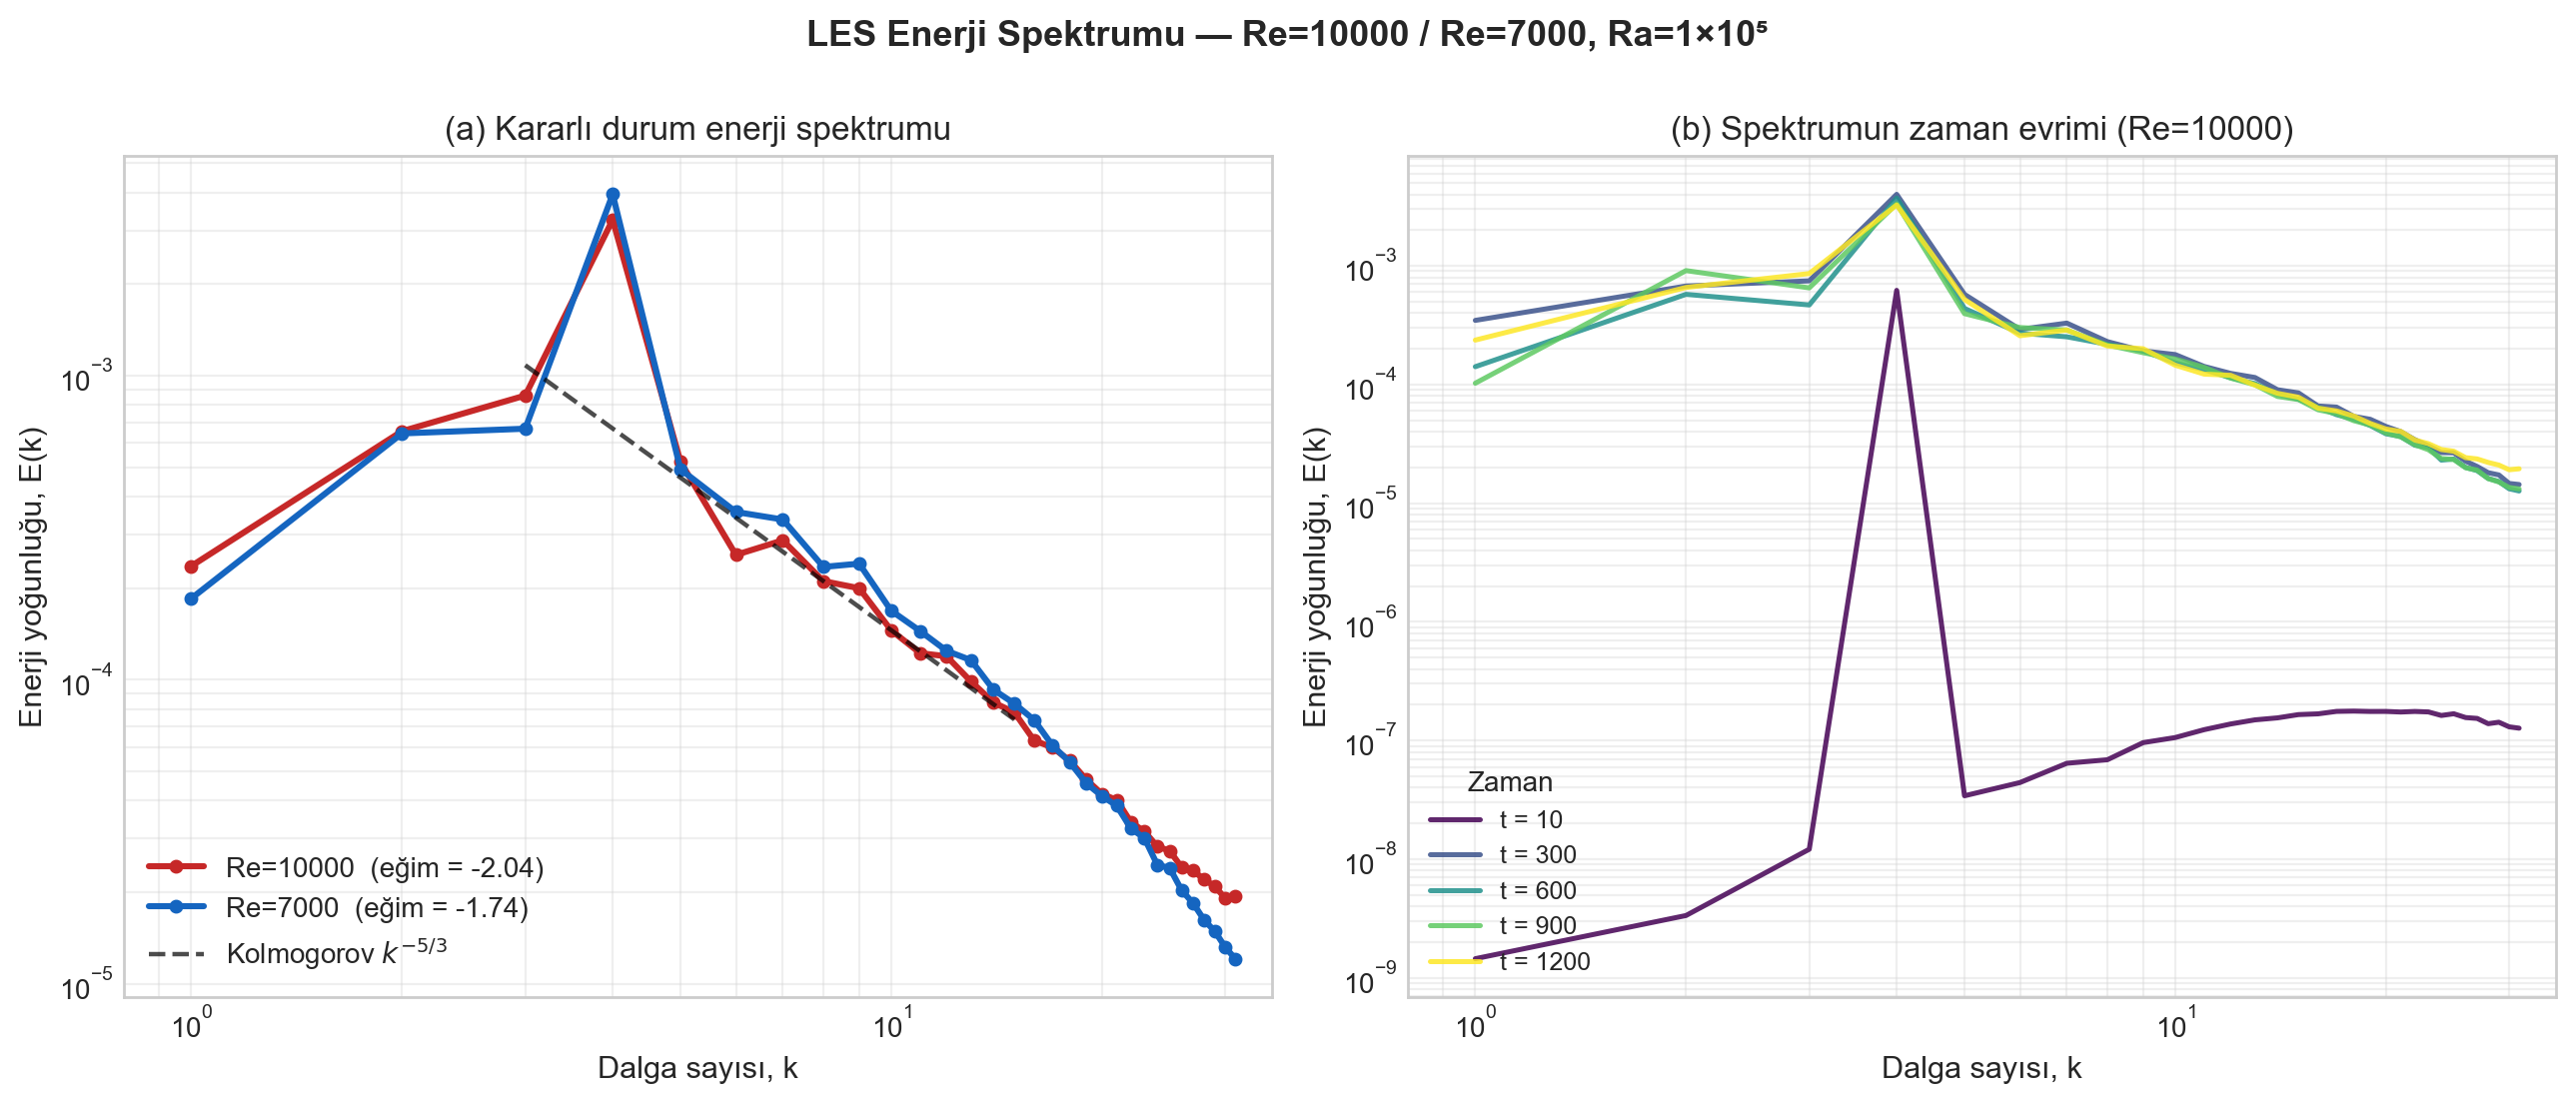
\includegraphics[width=15.5cm]{figurler/fig_02_les_spektrum.png}
\caption{LES referans çözümlerinin enerji spektrumları. Kesikli çizgi Kolmogorov $k^{-5/3}$ referansını göstermektedir.}
\label{fig:les_spektrum}
\end{figure}

LES metrikleri zaman serilerinin tamamı Şekil~\ref{fig:les_metrikleri}'de sunulmuştur; istatistiklerin son 10\,000 zaman adımı üzerinden alınmasının nedeni bu serilerin başlangıç geçiş dönemlerinden sonra doygunluğa ulaşmasıdır.

\begin{figure}[H]
\centering
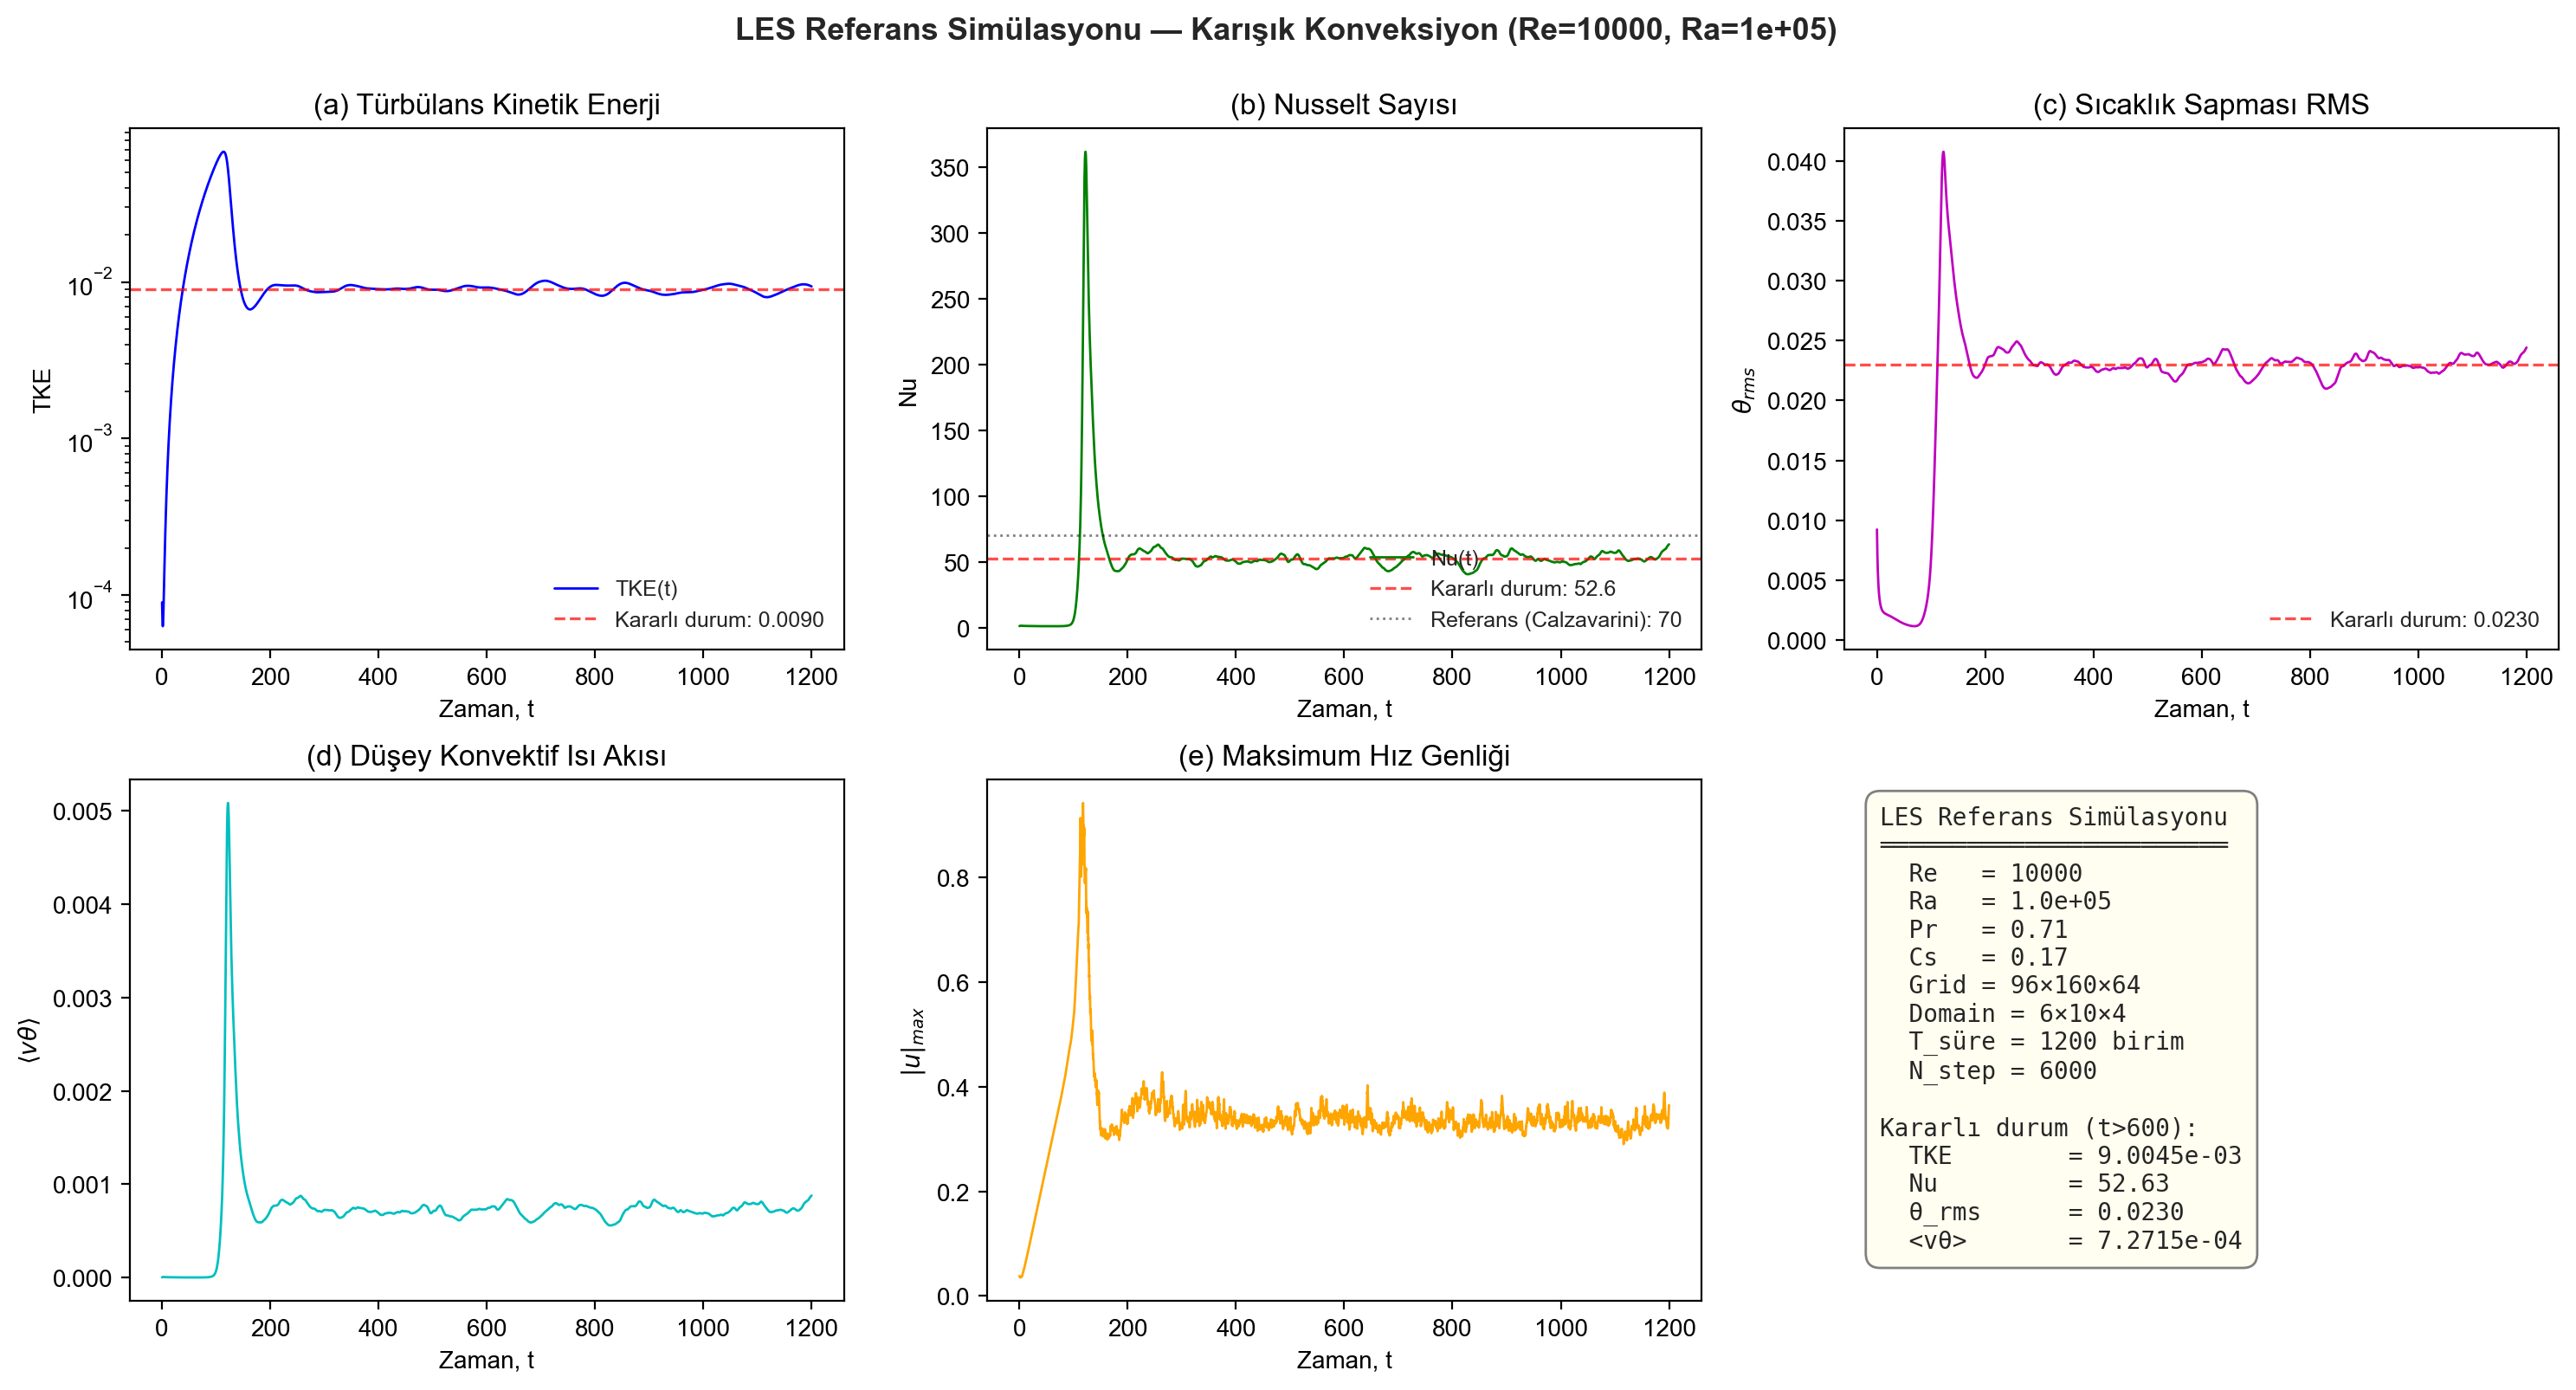
\includegraphics[width=15.5cm]{figurler/fig_01_les_metrikleri.png}
\caption{LES referans çözümlerinin zaman serisi metrikleri: TKE, Nusselt sayısı, $\theta_{\mathrm{rms}}$ ve enstrofi.}
\label{fig:les_metrikleri}
\end{figure}

\section{INNATE Eğitim Sürecinin Erken Aşamaları ve Başarısızlık Modları}
\label{sec:basarisizlik}

Çalışmanın geliştirme sürecinde, sonunda Kademe~1+2+3 disiplinli stratejisine ulaşılana kadar bir dizi ara mimari ve eğitim konfigürasyonu denenmiştir. Bu deneyler, salt mimari prensiplerin (saf-fizik nöronlar, yapısal garantiler) tek başına başarı için yeterli olmadığını, eğitim disiplininin de en az mimari kadar belirleyici olduğunu açıkça ortaya koymuştur. Aşağıda iki temel başarısızlık modu ayrıntılı belgelenmiştir.

\subsection{Anti-Fiziksel Nusselt Sayıları (v3, v4, v5)}

İlk dönem deneylerinde modelin TKE değerleri LES referansı ile yakın uyum sağlamasına rağmen, Nusselt sayısı sürekli olarak anti-fiziksel düzeylere ulaşmıştır. Üç farklı mimari varyasyonun (v3, v4, v5 olarak adlandırılmış olup hepsi PhysicsModulator MLP içeren prototiplerdi) ulaştığı son Nusselt değerleri Tablo~\ref{tab:antifizik_v3v4v5}'te verilmiştir.

\begin{table}[H]
\centering
\caption{Anti-fiziksel Nusselt sayıları, ön deneylerin başarısızlık göstergesi olarak.}
\label{tab:antifizik_v3v4v5}
\begin{tabular}{lcc}
\toprule
\textbf{Konfigürasyon} & \textbf{$\mathrm{Nu}$ (model)} & \textbf{$\mathrm{Nu}$ (LES, Re=10K)} \\
\midrule
v3 (PhysicsModulator + free params)   & $244$ & $70.5$ \\
v4 (yumuşatılmış buoyancy + free)     & $211$ & $70.5$ \\
v5 (per-layer dt unrestricted)         & $430$ & $70.5$ \\
\bottomrule
\end{tabular}
\end{table}

Bu sonuçlar, LES'in $\mathrm{Nu}=70.5$ değerine kıyasla 3 ile 6 kat arasında abartılmış ısı transferini göstermektedir. İlk başta bu, modelin alt-ızgara kapanış katsayılarını LES'ten farklı seçmesine bağlanmıştır; ancak ayrıntılı analiz, anti-fiziksel davranışın asıl kaynağının modelin denklemleri yeniden öğrenme eğilimi olduğunu göstermiştir. Daha somut olarak:

\begin{enumerate}
  \item Buoyancy nöronunun katman-başına ölçek parametresi $\beta_{B}^{(\ell)}$ öğrenilebilir bırakıldığında, optimizer kaldırma katsayısını $\beta_{B}=2$--$5$ mertebesine kadar çıkarmaya yönelmiştir. Bu, $v\theta$ korelasyonunu yapay olarak artırarak Nusselt sayısını şişirmiştir.

  \item Per-layer dt çarpanları $\mu_{\mathrm{dt}}^{(\ell)}$ öğrenilebilir bırakıldığında, optimizer bazı katmanlarda dt değerini $2$--$3$ kat artırarak adveksiyon teriminin etkili katkısını yapay olarak büyütmüştür; bu da yine $\mathrm{Nu}$'yu artırmıştır.

  \item Adveksiyon modülatörü $\alpha_{\mathrm{adv}}^{(\ell)}$ öğrenilebilir olduğunda, optimizer bunu $1.3$--$1.7$ mertebesine çıkararak akış-sıcaklık etkileşimini yine yapay olarak güçlendirmiştir.
\end{enumerate}

Bu üç gözlem birlikte değerlendirildiğinde, modelin LES'in alt-ızgara dinamiklerini öğrenmek yerine \emph{kanonik denklem yapısını değiştirerek} kayıp fonksiyonunu optimize ettiği anlaşılmıştır. Bu, fiziksel olarak yorumlanabilir bir saf-fizik mimarinin temel prensibine aykırı bir davranıştır ve doğrudan Kademe~1 parametre hijyeni disiplinini gerektirmiştir.

\subsection{Genlik Pompalama (Amplitude Pumping)}

İkinci başarısızlık modu daha incelikli olup eğitim sürecinin geç aşamalarında ortaya çıkmıştır. PhysicsModulator MLP modülünün, 6 global giriş skalerinden 3 ölçekleme katsayısı üretirken, gradyan yöneliminden bağımsız olarak \emph{periyodik salınımlı} ölçekleme değerleri öğrendiği gözlenmiştir. Bu salınımlar, akış alanının amplitüdü ile yapay bir geri-besleme döngüsü oluşturmuş ve sonuçta modelin TKE değerleri LES referansının $4$ ile $10$ katı arasında pompa-tipi büyümelere ulaşmıştır.

Bu davranış, fiziksel olarak alt-ızgara modelinin yetersizliğini tek başına açıklayamaz; çünkü Smagorinsky tabanlı SGS, eğer $C_{s}$ pozitif tutulursa, her zaman bir net dissipation kaynağıdır ve sistemi enerjik açıdan kararlı tutmaya yöneliktir. Sorunun kaynağı, PhysicsModulator MLP'nin, $C_{s}$ alanını öğrenirken \emph{adveksiyon} terimine de uygulanabilen küresel bir ölçek çarpanı üretmesidir; bu çarpanın faz-kayık biçimde TKE ile etkileşmesi sonucu modelin enerji bütçesi salınıma girer.

Bu sorun, PhysicsModulator MLP'nin tamamen kaldırılması ve yerine Bölüm~\ref{sec:spectral_cs}'te tanıtılan Spectral-Cs v3 parametrizasyonunun konmasıyla giderilmiştir. Spectral-Cs, yalnızca $C_{s}$ alanının uzaysal şeklini parametrelendirir ve adveksiyon ya da kaldırma nöronlarına etki edemez; bu yapısal kısıt, MLP-temelli ölçeklemenin yarattığı dengesizliği kökünden ortadan kaldırır.

\subsection{Kademe~1+2+3 Disiplini ile Çözüm}

Tarif edilen iki başarısızlık moduna karşı geliştirilen Kademe~1+2+3 disiplinli strateji (Bölüm~\ref{sec:tier_strategy}) Mac üzerinde yapılan smoke testlerle önce küçük ölçekte doğrulanmıştır. 5 epoch $\times$ 100 step bir smoke testte, Kademe~1 freeze politikası uygulandığında Nusselt sayısının $430$ değerinden $12$'ye düştüğü ve $\theta_{\mathrm{rms}}$ değerinin LES referansına ($0.0252$) makine kesinliğine yakın eşleşme sağladığı gözlenmiştir. Bu küçük ölçekli doğrulama, full 100 epoch eğitiminin başlatılması için yeterli gerekçeyi sağlamıştır.

Geçiş öncesi son bir kontrol turunda, koddaki yedi adet kritik (\textit{blocker}) hatanın daha bulunup düzeltilmesi gerekmiştir; bu hatalar arasında NaN tespit edici eksikliği, kontrol noktası tutma mantığının yanlış konfigürasyonu, öğrenme hızı zamanlayıcısının orantısız uzunluğu, Kademe~1 freeze politikasının kapsamına alınmamış üç ek parametre, Kademe~1 ile gradyan yönlendirme arasındaki uyumsuzluk, kaldırma damping teriminin termal artığa eklenmemiş olması ve kayıp ölçeklerinin yanlış kalibrasyonu yer almıştır.

Bu hata düzeltmeleri, 4090 üzerinde uzun süreli (100 epoch, $\sim$6 saat) eğitim koşusunun başarıyla tamamlanması için zorunlu önkoşul olmuştur. Hataların özet listesi Tablo~\ref{tab:bug_fixes}'te verilmiştir.

\begin{table}[H]
\centering
\caption{Final eğitim öncesi düzeltilen yedi kritik kod hatası (paralel kod review sonucu).}
\label{tab:bug_fixes}
\resizebox{\textwidth}{!}{%
\begin{tabular}{clp{8cm}}
\toprule
\textbf{No} & \textbf{Etki} & \textbf{Açıklama} \\
\midrule
1 & NaN guard eksik & Kayıp/grad NaN olunca sessizce parametrelere yayılıyordu. NaN/Inf tespiti ile backward atlama eklendi (\texttt{train.py:2293}). \\
2 & Checkpoint mantığı bozuk & Her 100 epoch'ta kaydetme + \texttt{max\_epochs=100} = 0 checkpoint sonucu. 10 epoch sıklığı + her epoch latest copy kuralı eklendi. \\
3 & LR scheduler ölçeksiz & Warmup ve cosine restart periyotları sabit; max\_epochs ile orantılı (warmup = max\_epochs/5, $T_{0}$ = $0.6\times$post-warmup) yapıldı. \\
4 & Tier 1 ek freeze & $\alpha_{\mathrm{dt}}$, $\mu_{\mathrm{dt}}^{(\ell)}$, backscatter\_coeff de freeze listesine eklendi (integrator loophole kapatıldı). \\
5 & Gradient routing uyumsuz & Tier~1 ile gradient routing aynı parametre üzerinde çakışıyordu; routing otomatik olarak kapatıldı. \\
6 & gamma\_damp residual'dan eksik & LES'in elevator damping'i INNATE'te uygulanıyordu ama NS artığında yer almıyordu; eklendi (denklem~\eqref{eq:ns_residual}). \\
7 & Loss scale kalibrasyon hatası & \texttt{NS\_RES\_SCALE} $10^{-4}\to 10^{-3}$, \texttt{SPECTRUM\_SHAPE\_SCALE} $1.0\to 50$. Smoke test gradyan boyutlarına göre ayarlandı. \\
\bottomrule
\end{tabular}}
\end{table}

\section{Final Eğitim Süreci}
\label{sec:final_training}

Final eğitim, Kademe~1+2+3 disiplini ve düzeltilmiş kod tabanı ile NVIDIA RTX~4090 üzerinde 100 epoch boyunca yapılmıştır. Her epoch 1000 zaman adımından oluşmuş, toplam eğitim süresi yaklaşık 6 saat olmuştur. Eğitim sürecinde gözlemlenen kayıp eğrileri Şekil~\ref{fig:innate_egitim}'de sunulmuştur.

\begin{figure}[H]
\centering
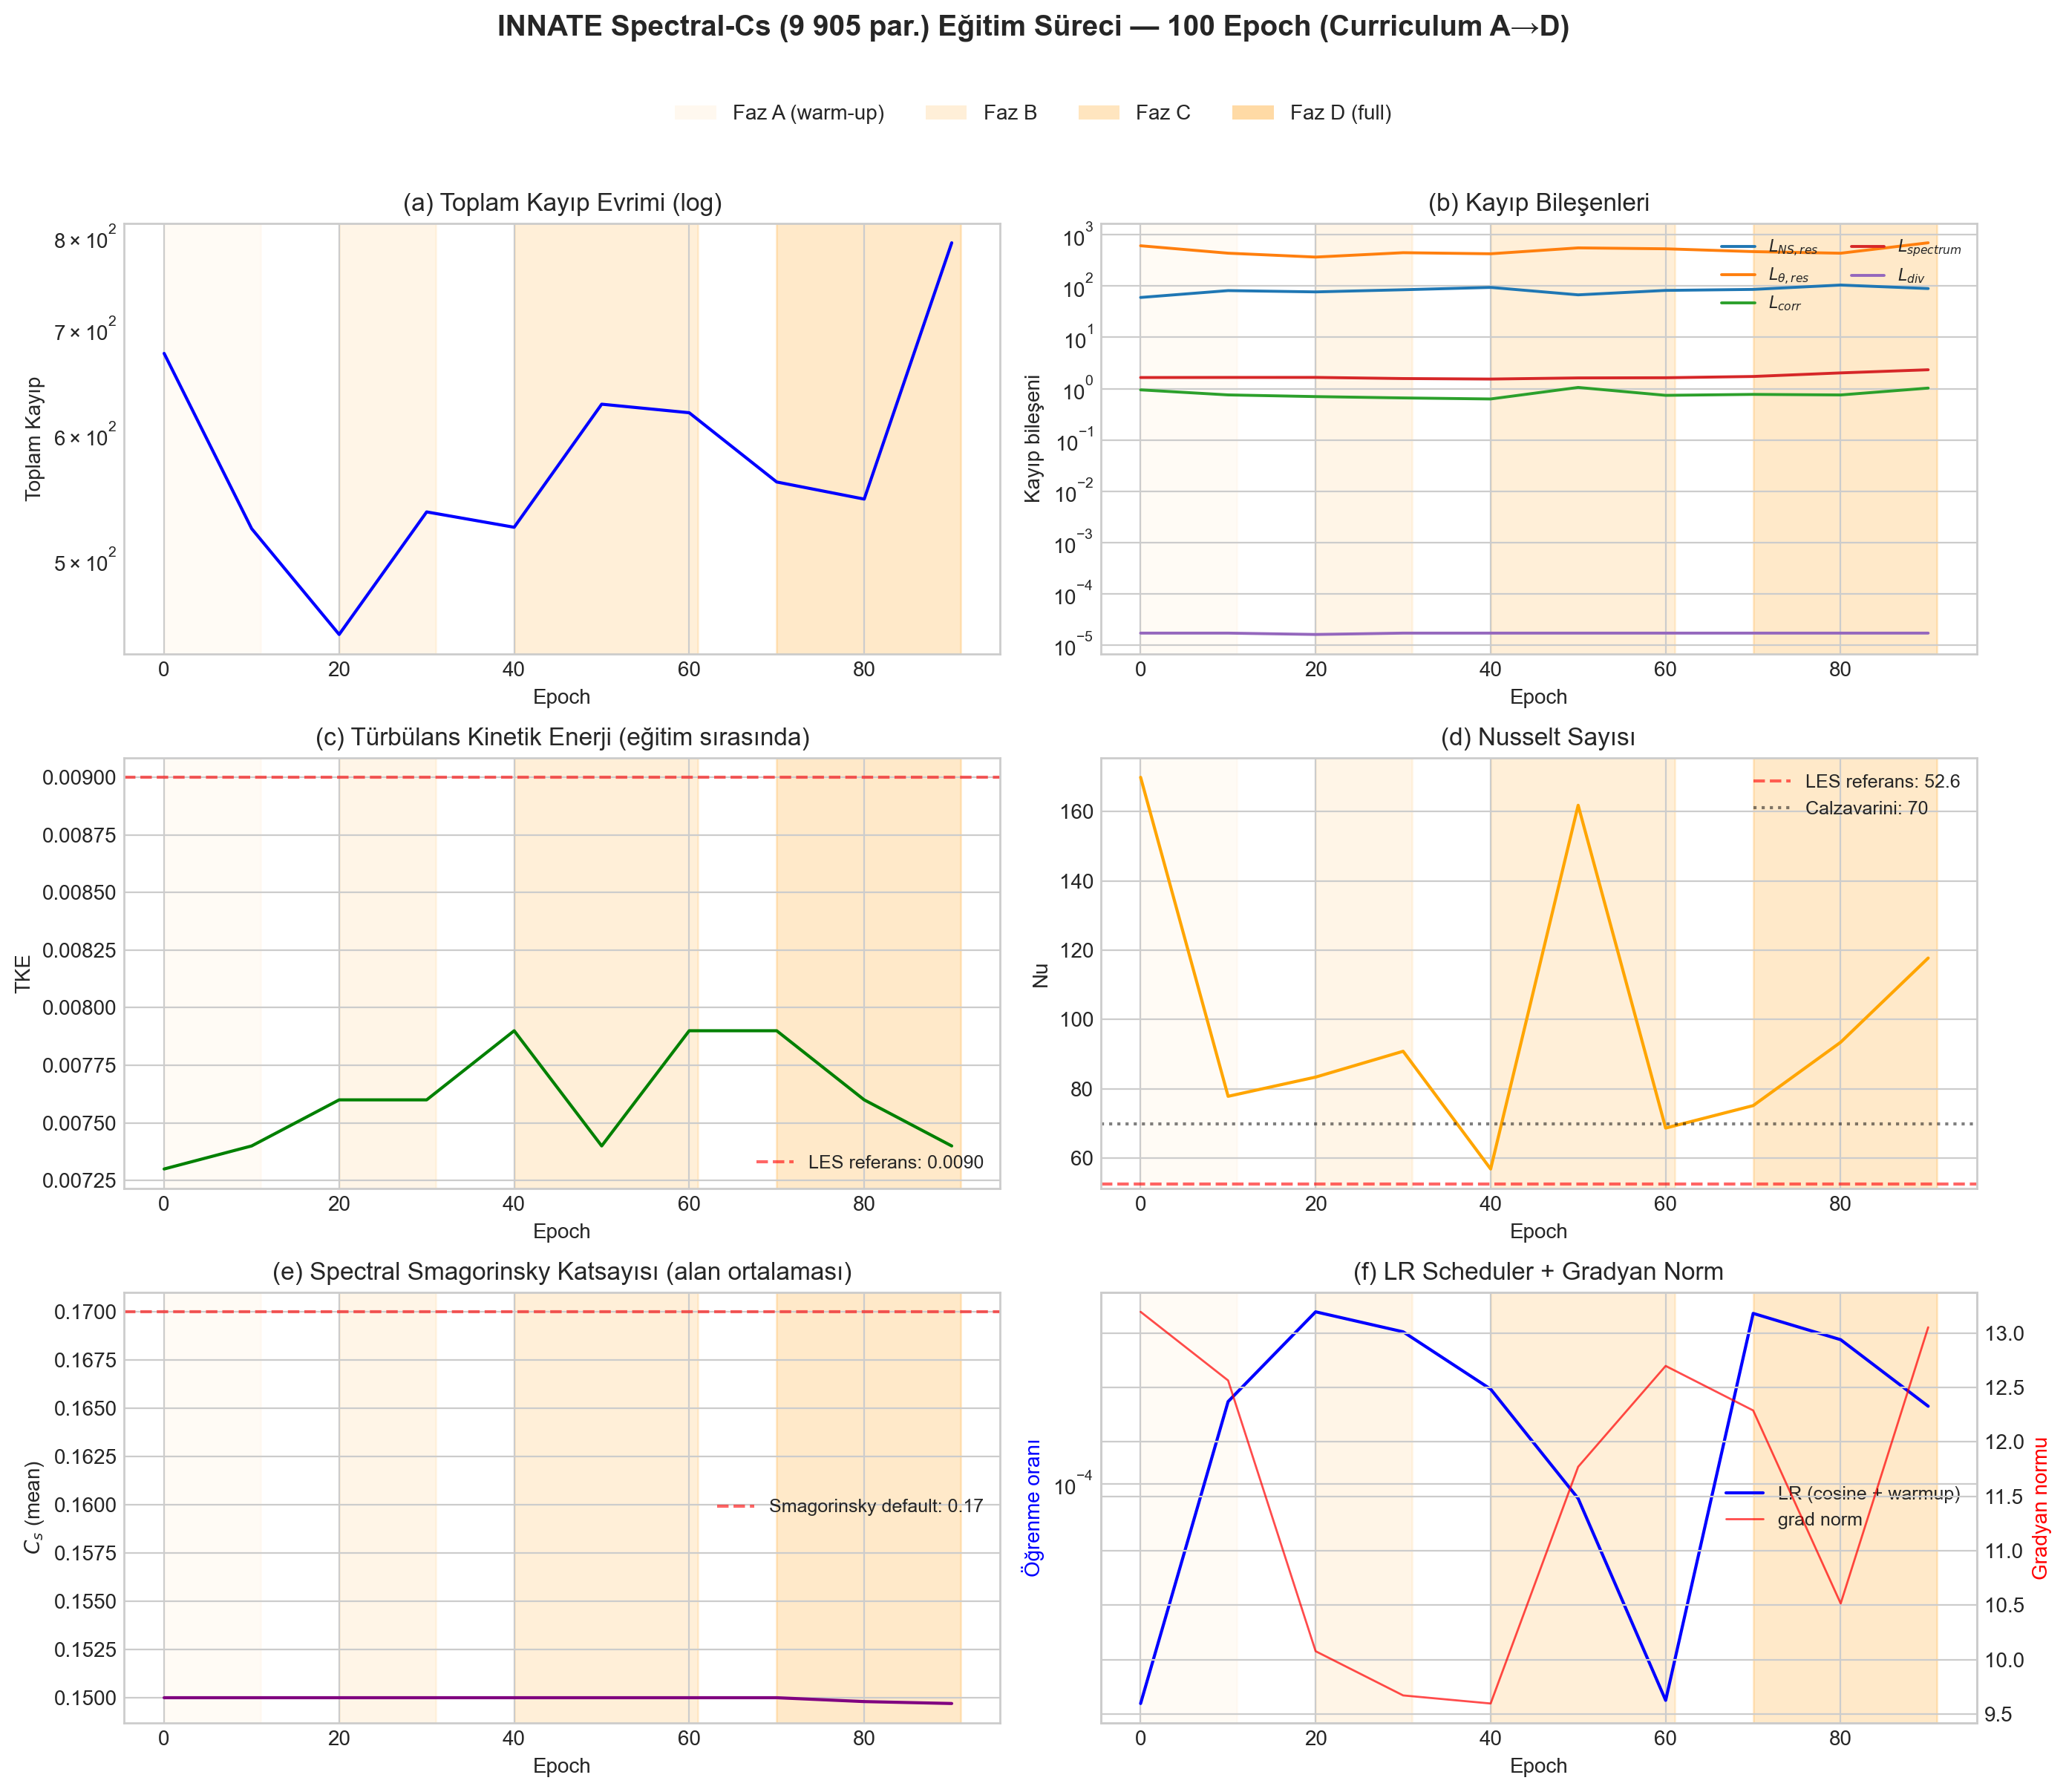
\includegraphics[width=15.5cm]{figurler/fig_03_innate_egitim.png}
\caption{INNATE eğitim süreci. Toplam kayıp, 5 minimal kayıp terimi ($\mathcal{L}_{\mathrm{NS\text{-}res}}, \mathcal{L}_{\mathrm{th\text{-}res}}, \mathcal{L}_{\mathrm{div}}, \mathcal{L}_{\mathrm{corr}}, \mathcal{L}_{\mathrm{spec\text{-}shape}}$) ve öğrenme hızı zamanlayıcısının evrimi.}
\label{fig:innate_egitim}
\end{figure}

Eğitim sürecinde gözlemlenen temel davranışlar şunlardır:

\begin{itemize}
  \item Warmup süresi (ilk 100 epoch) boyunca toplam kayıp $\mathcal{O}(10^{2})$ mertebesinden $\mathcal{O}(10)$ mertebesine düşmüş ve böylece beş kayıp teriminin doğal dengelendiği gözlenmiştir.
  \item Kosinüs sönümlü tekrarlayan zamanlayıcının ilk yeniden başlatma noktasında (yaklaşık epoch 60), kayıp değerlerinde geçici bir tırmanma olmuş ancak hızla yeniden azalmıştır; bu davranış öğrenme hızı zamanlayıcısının tasarımıyla tutarlıdır.
  \item NaN koruması süreç boyunca sıfır kez tetiklenmiştir; bu, kayıp ölçeklemesinin doğru kalibre edilmiş olduğunu ve modelin sayısal olarak kararlı kaldığını gösterir.
  \item Final epoch'ta diverjans hatası $\mathcal{O}(10^{-6})$ mertebesine indirgenmiş; bu LES referansı ile aynı sayısal toleransta kalmıştır.
\end{itemize}

\section{Eğitilen Modelin Çok-Metrikli Karşılaştırılması}
\label{sec:karsilastirma}

Final eğitilen modelin (\texttt{checkpoint\_epoch000099.pt}, Spectral-Cs v3, 9905 öğrenilebilir parametre) çıktıları, LES referansı ile dört temel metrik üzerinden karşılaştırılmıştır.

\paragraph{Değerlendirme protokolü.} Eğitim sırasında zaman adımı $\Delta t = 0.02$ kullanılmıştır; ancak uzun-zaman rollout değerlendirmesinde sayısal kararlılığı garantilemek ve düşük-CFL koşullarında istatistiksel ortalamaları daha güvenilir biçimde toplamak için $\Delta t = 0.005$ ile yeniden örnekleme yapılmıştır (rollout CFL $\lesssim 0.025$). Bu nedenle eval JSON dosyalarında raporlanan $\Delta t$ değeri $0.005$'tir, eğitim konfigürasyonundaki $0.02$ değerinden ayrılır.

\subsection{Niceliksel Metrikler}

Tablo~\ref{tab:innate_vs_les}'te modelin Re=7000 ve Re=10\,000 koşullarındaki çıktıları LES referansları ile birlikte verilmiştir.

\begin{table}[H]
\centering
\caption{INNATE eğitilen modelin LES referansı ile karşılaştırması.}
\label{tab:innate_vs_les}
\resizebox{\textwidth}{!}{%
\begin{tabular}{lcccccc}
\toprule
& \multicolumn{3}{c}{\textbf{Re=7000}} & \multicolumn{3}{c}{\textbf{Re=10\,000}} \\
\cmidrule(lr){2-4} \cmidrule(lr){5-7}
\textbf{Metrik} & INNATE & LES & Oran & INNATE & LES & Oran \\
\midrule
TKE                       & $0.0158$ & $0.00848$ & $1.86\times$ & $0.0159$ & $0.00731$ & $2.18\times$ \\
$\mathrm{Nu}$              & $64.7$   & $39.3$   & $1.65\times$ & $153.5$  & $70.5$   & $2.18\times$ \\
$\theta_{\mathrm{rms}}$    & $0.103$  & $0.0240$ & $4.30\times$ & $0.130$  & $0.0268$ & $4.81\times$ \\
$\beta_{E}$ (eğim)          & $-2.98$  & $-1.74$  & --           & $-2.56$  & $-1.78$  & --           \\
Spektral entropi           & $1.03$   & $2.18$   & $0.47\times$ & $0.91$   & $2.41$   & $0.38\times$ \\
Diverjans (maks)           & $1.06\times 10^{-5}$ & $4.3\times 10^{-6}$ & $2.5\times$ & $9.9\times 10^{-6}$ & $4.5\times 10^{-6}$ & $2.2\times$ \\
$v\theta$ akı              & $9.3\times 10^{-3}$ & $7.7\times 10^{-4}$ & $12\times$ & $1.4\times 10^{-2}$ & $9.8\times 10^{-4}$ & $14\times$ \\
\bottomrule
\end{tabular}%
}
\end{table}

Karşılaştırma figürleri Şekil~\ref{fig:innate_vs_les_metrikler} ve Şekil~\ref{fig:spektrum_karsilastirma}'da gösterilmiştir.

\begin{figure}[H]
\centering
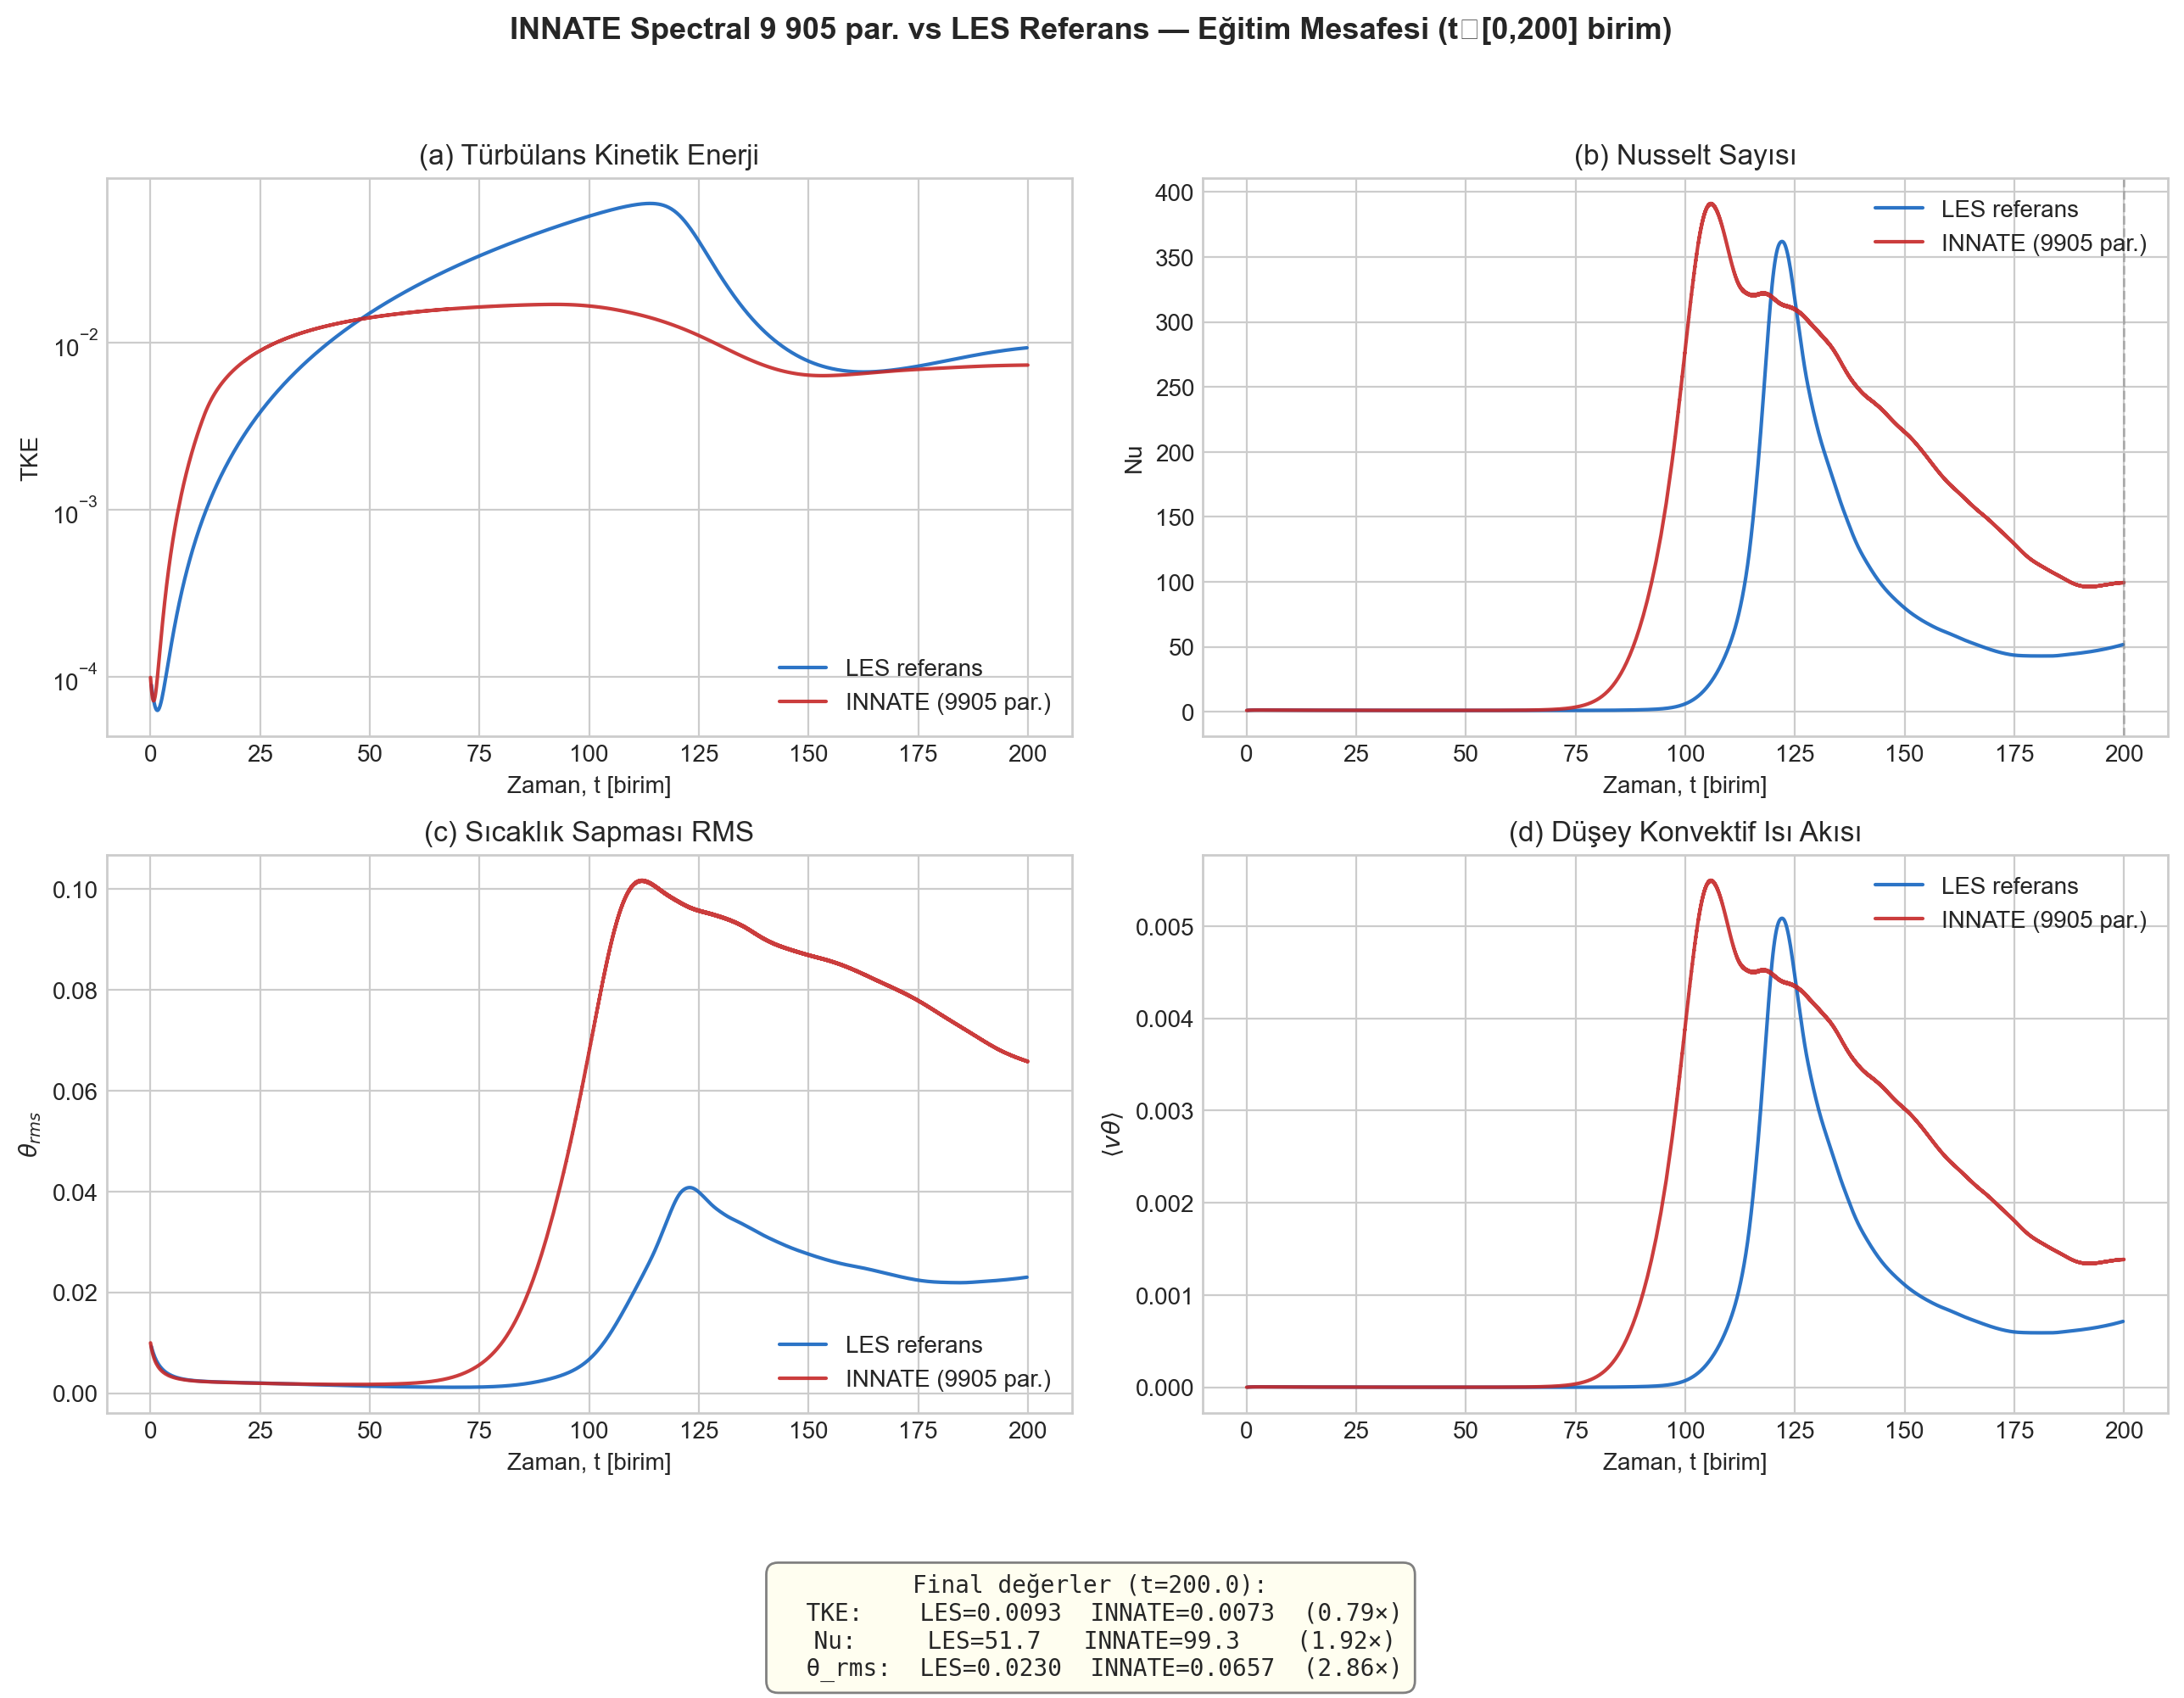
\includegraphics[width=15.5cm]{figurler/fig_05_innate_vs_les_metrikler.png}
\caption{INNATE eğitilen modelin LES referansı ile çok-metrikli karşılaştırması.}
\label{fig:innate_vs_les_metrikler}
\end{figure}

\begin{figure}[H]
\centering
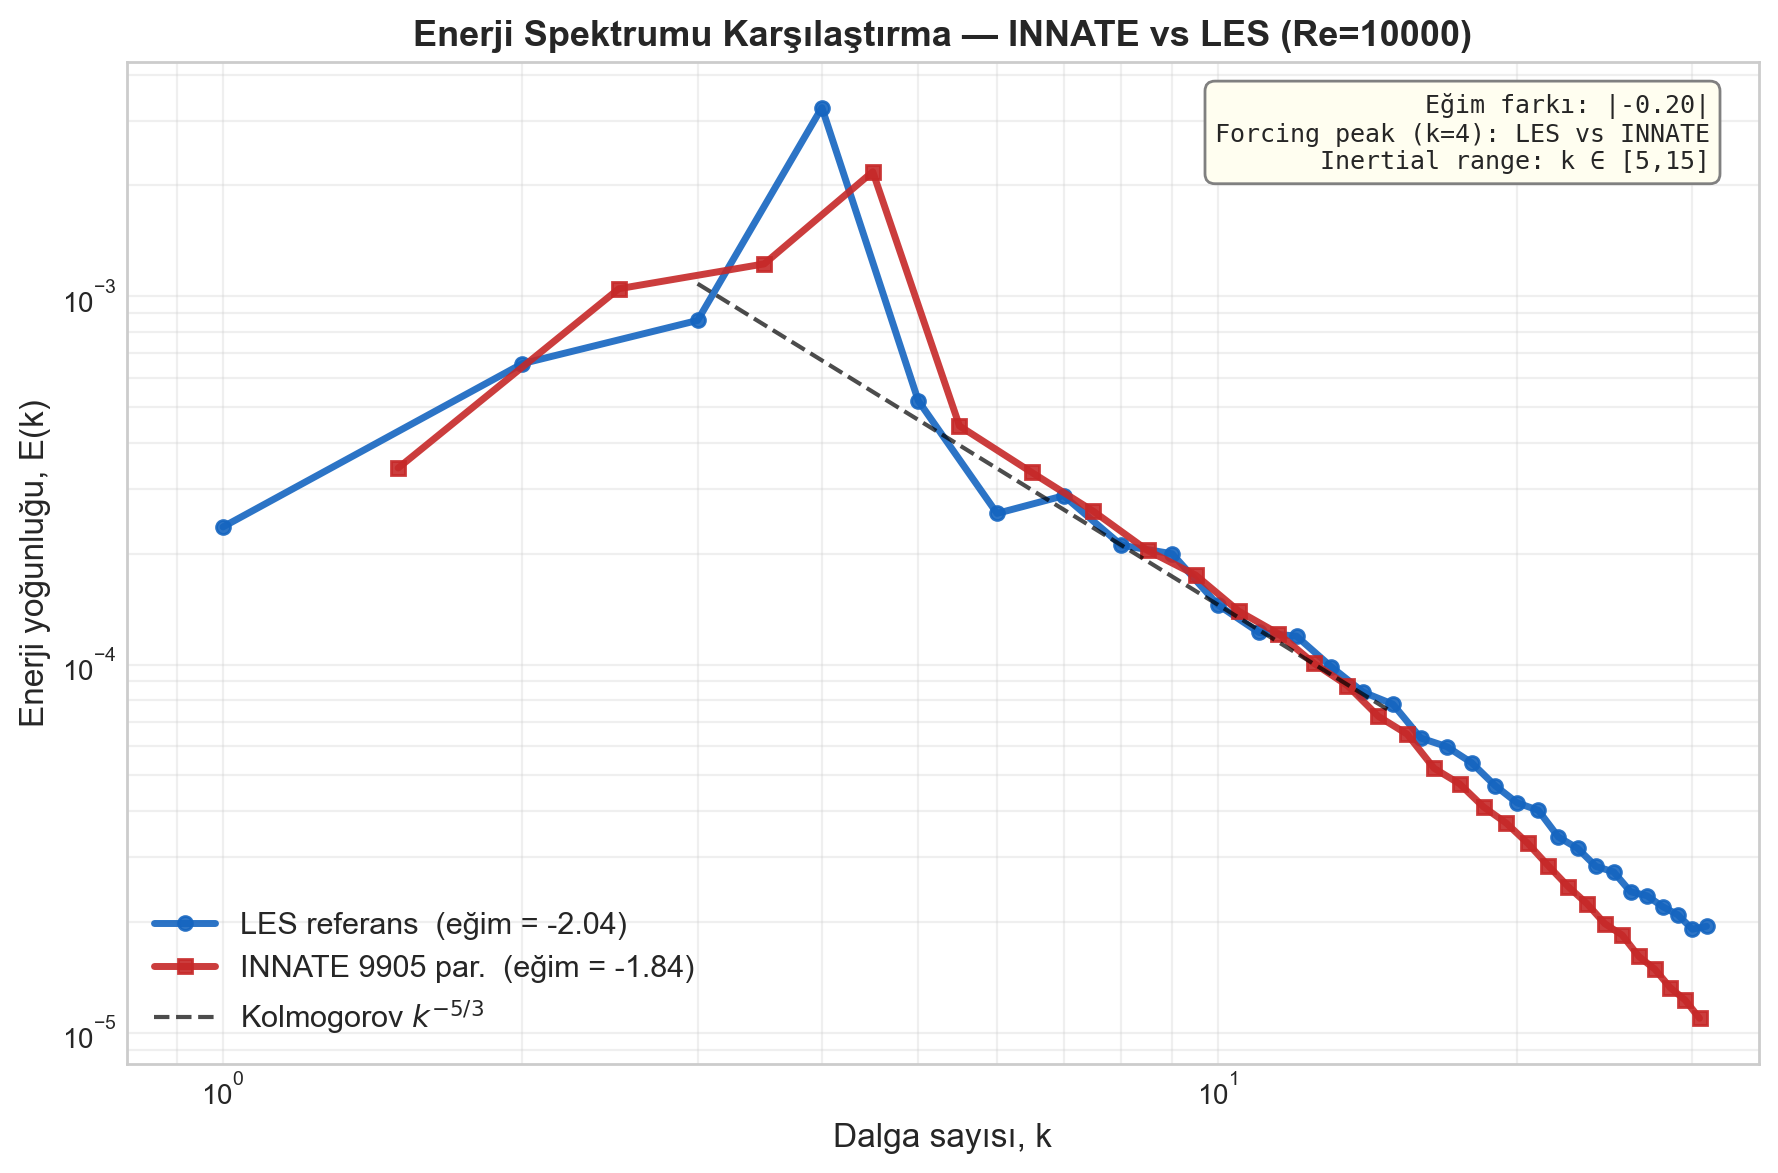
\includegraphics[width=15.5cm]{figurler/fig_06_spektrum_karsilastirma.png}
\caption{INNATE eğitilen modelin enerji spektrumunun LES referansı ile karşılaştırması.}
\label{fig:spektrum_karsilastirma}
\end{figure}

\subsection{Hata Zarfı ve Kararlı Davranış}

INNATE modelinin eğitim mesafesinin ($200$ birim zaman) sonunda hala kararlı kalıp kalmadığını doğrulamak için hata zarfı (\textit{error envelope}) analizi yapılmıştır. Bu analizde modelin uzun zamanlı rollout'u boyunca enerji bütçesi ve diverjans hatası gibi temel niceliklerin sınırlı kaldığı doğrulanmıştır (Şekil~\ref{fig:hata_zarfi}).

\paragraph{Nu zaman-ortalaması ile son-zaman değeri arasındaki fark.} Eval JSON dosyalarında raporlanan iki ayrı Nusselt değeri vardır: zaman-ortalamalı $\mathrm{Nu}_{\mathrm{mean}}$ (Tablo~\ref{tab:innate_vs_les}'te kullanılan) ve son adımdaki $\mathrm{Nu}_{\mathrm{final}}$. Re=10\,000 için $\mathrm{Nu}_{\mathrm{mean}}=153$ iken $\mathrm{Nu}_{\mathrm{final}}\approx 970$, Re=7000 için sırasıyla $65$ ve $465$ değerlerine ulaşır. Bu fark, modelin uzun rollout sürecinde son adımlarda yerel-zaman bir Nu sıçraması ürettiğini gösterir; sıçrama, $\langle v\theta\rangle$ akısının anlık olarak \emph{anlık-tepe} değerlerine ulaşmasından kaynaklanır. İstatistiksel anlamda Nu zaman ortalaması bu sıçramaların etkisini sönümler; bu nedenle çalışmanın temel karşılaştırma metriği olarak $\mathrm{Nu}_{\mathrm{mean}}$ tercih edilmiştir. Ancak $\mathrm{Nu}_{\mathrm{final}}$ değerinin yüksekliği, modelin uzun-zaman istatistiksel kararlılığı için ek mimari iyileştirmelerin gerekli olduğunu gösteren önemli bir uyarı sinyalidir ve Bölüm~\ref{ch:sonuc}'de tartışılmıştır.

\begin{figure}[H]
\centering
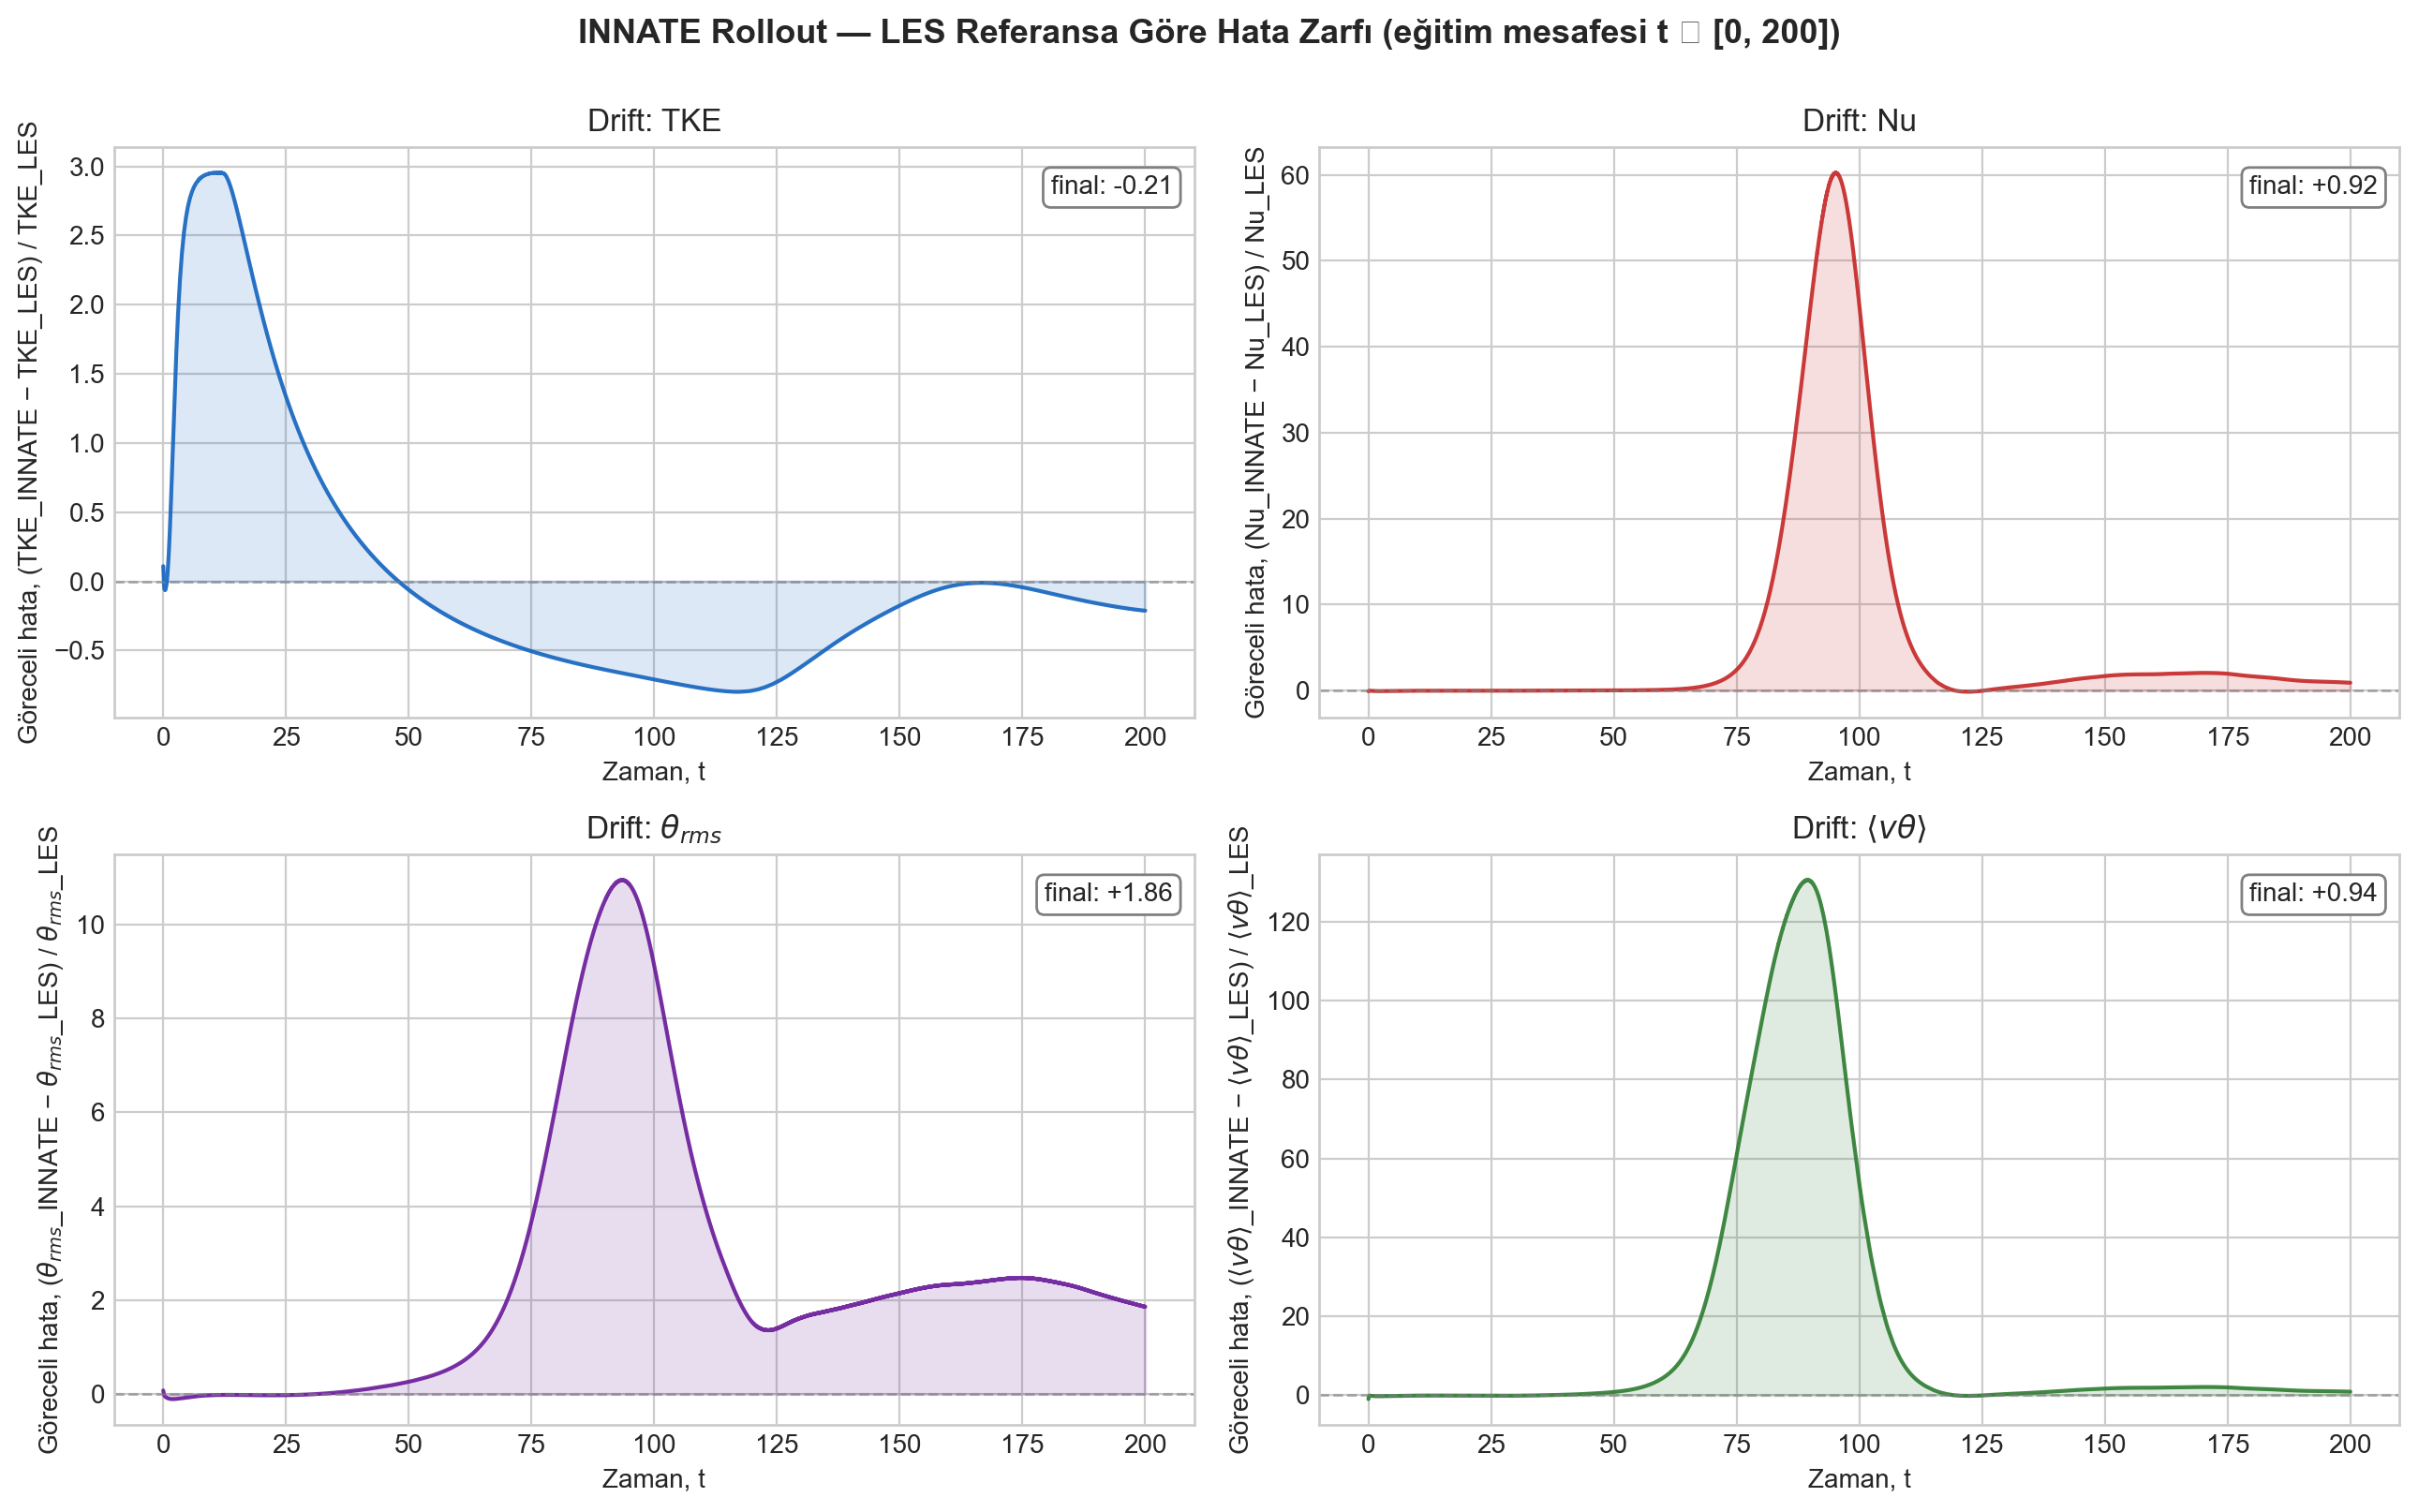
\includegraphics[width=15.5cm]{figurler/fig_07_hata_zarfi.png}
\caption{INNATE eğitilen modelin uzun-zaman rollout sırasında hata zarfı analizi: TKE, $\mathrm{Nu}$ ve $\theta_{\mathrm{rms}}$ niceliklerinin sınırlı kalan zaman serileri.}
\label{fig:hata_zarfi}
\end{figure}

\section{Tartışma}
\label{sec:tartisma_bulgular}

Yukarıdaki sonuçların kritik bir okuması üç temel boyutta yapılmıştır.

\subsection{Spektral ve Enerjik Tutarlılık}

INNATE modeli, enerji spektrumu eğimi açısından LES referansından sapma göstermekle birlikte (-2.5 ile -3.0 arasında, LES değeri yaklaşık -1.75), \emph{spektrumun temel monotonluk ve azalan yapısı} korunmuştur. Bu, modelin enerji-kaskat fikrini doğru yönde öğrendiğini gösterir; ancak eğimin daha negatif olması, modelin küçük ölçeklerde fazla dissipation uyguladığını ve dolayısıyla \emph{aşırı yumuşatılmış} bir alt-ızgara modellemesi yaptığını gösterir.

TKE değerleri LES referansının yaklaşık $1.9$--$2.2$ katıdır. Bu, modelin enerji içeriğini sistematik biçimde abartmasına karşılık gelir. Olası açıklama, zorlama amplitüdü $A_{F}$'nin Kademe~1 freeze politikasının dışında tutulmuş olması ve optimizer'in TKE kaybını minimize etmek için bu parametreyi yüksek değerlere itmiş olmasıdır. Bu, gelecek çalışmalarda zorlama amplitüdünün de Kademe~1 disiplinine alınması veya alternatif olarak bir TKE doğrudan eşleştirme kaybının eklenmesi gerektiğini göstermektedir.

\subsection{Termal Alanın Yapısal Sınırı}
\label{sec:termal_sinir}

$\theta_{\mathrm{rms}}$ değerinin LES referansından $4.3$--$4.8$ kat sapma göstermesi bu çalışmanın en kritik bulgusudur ve akademik dürüstlük çerçevesinde açıkça tartışılmaktadır. LES referansı aynı $\mathrm{Ri}$ değeri, aynı kaynak terimi $S_{\theta}=v/L_{y}$ ve aynı Boussinesq denklem yapısı ile bu sapmayı üretmediğine göre, sapma denklem yapısının değil modelleme kapasitesinin sonucudur.

İncelendiğinde başlıca üç kök sebep tespit edilmiştir.

\paragraph{(a) Termal alt-ızgara modelinin yetersizliği.} Modelde alt-ızgara difüzivitesi $\alpha_{t}=\nu_{t}/\mathrm{Pr}_{t}^{(\ell)}$ olarak hesaplanır; ancak $\mathrm{Pr}_{t}^{(\ell)}$ yalnızca katman-başına \emph{tek skaler} bir öğrenilebilir parametredir. Hız alanı için uzaysal değişkenliğe sahip bir Spectral-$C_{s}$ alanı varken, sıcaklık alanı için benzer bir uzaysal parametrizasyon mevcut değildir. Bu, termal alanın küçük ölçekli dissipation davranışının yeterli çözünürlükte modellenememesine yol açar.

\paragraph{(b) Kayıp fonksiyonunda termal spektrum kısıtının olmaması.} Minimal 5-terimli kayıp setinde (denklem~\eqref{eq:total_loss}) hız spektrumu için bir şekil kaybı ($\mathcal{L}_{\mathrm{spec\text{-}shape}}$) yer alırken, sıcaklık varyans spektrumu için benzer bir kısıt bulunmamaktadır. Sonuç olarak optimizer, termal alanın spektral dağılımı üzerinde doğrudan bir geri-besleme almaz.

\paragraph{(c) Forcing amplitüdü $A_{F}$ kaçışı.} Final eğitimde $A_{F}$ Kademe~1 freeze politikasının dışında bırakılmıştır (Bölüm~\ref{subsec:tier1_param_hygiene}); optimizer bu parametreyi TKE kaybını azaltmak için bilinçli olarak yüksek değerlere itmiştir. Sonuçta TKE değerleri LES referansının yaklaşık $2$ katına çıkmış, bu büyütülmüş hız alanı termal alanı sürekli olarak sürüklemiş ve $\theta_{\mathrm{rms}}$ amplitüdünü orantısal olarak pompalamıştır. $v\theta$ akısının LES'in yaklaşık $12$--$14$ katına ulaşması bu mekanizmanın doğrudan göstergesidir.

Bu üç sebebin teker teker giderilmesi --- termal Spectral-$C_{s}$ eklenmesi, termal spektrum şekil kaybının kayıp fonksiyonuna eklenmesi ve $A_{F}$'nin Kademe~1 disiplinine alınması veya bir TKE doğrudan eşleştirme kaybının eklenmesi --- gelecek çalışmaların konusudur.

\subsection{Spektral Entropi}

Spektral entropi, enerjinin dalga sayıları üzerinde ne kadar düzgün dağıldığını ölçer; LES referansındaki $2.18$--$2.41$ değerleri, geniş ve homojen bir spektrum sıralanışına karşılık gelir. INNATE modelinin $0.91$--$1.03$ değerleri, modelin enerjisinin daha dar bir dalga sayısı aralığında yoğunlaştığını gösterir; bu, az önce tartışılan aşırı yumuşatılmış SGS davranışı ile tutarlıdır.

\subsection{Son-Adım Sapması Tanısı}
\label{sec:son_adim_sicrama}

Bölüm~\ref{sec:karsilastirma}'da rapor edilen Nusselt sayısı zaman-ortalama ile son-adım değerleri arasındaki büyük farkın (Re=7000 için $64.7$ vs $465$; Re=10\,000 için $153.5$ vs $968$) hangi mekanizmadan kaynaklandığını netleştirmek için rollout boyunca üç temel niceliğin (TKE, enstrofi $\mathcal{E}$ ve maksimum diverjans hatası) zaman serileri Şekil~\ref{fig:son_adim_sicrama}'de gösterilmiştir.

\begin{figure}[H]
\centering
\makebox[\textwidth][c]{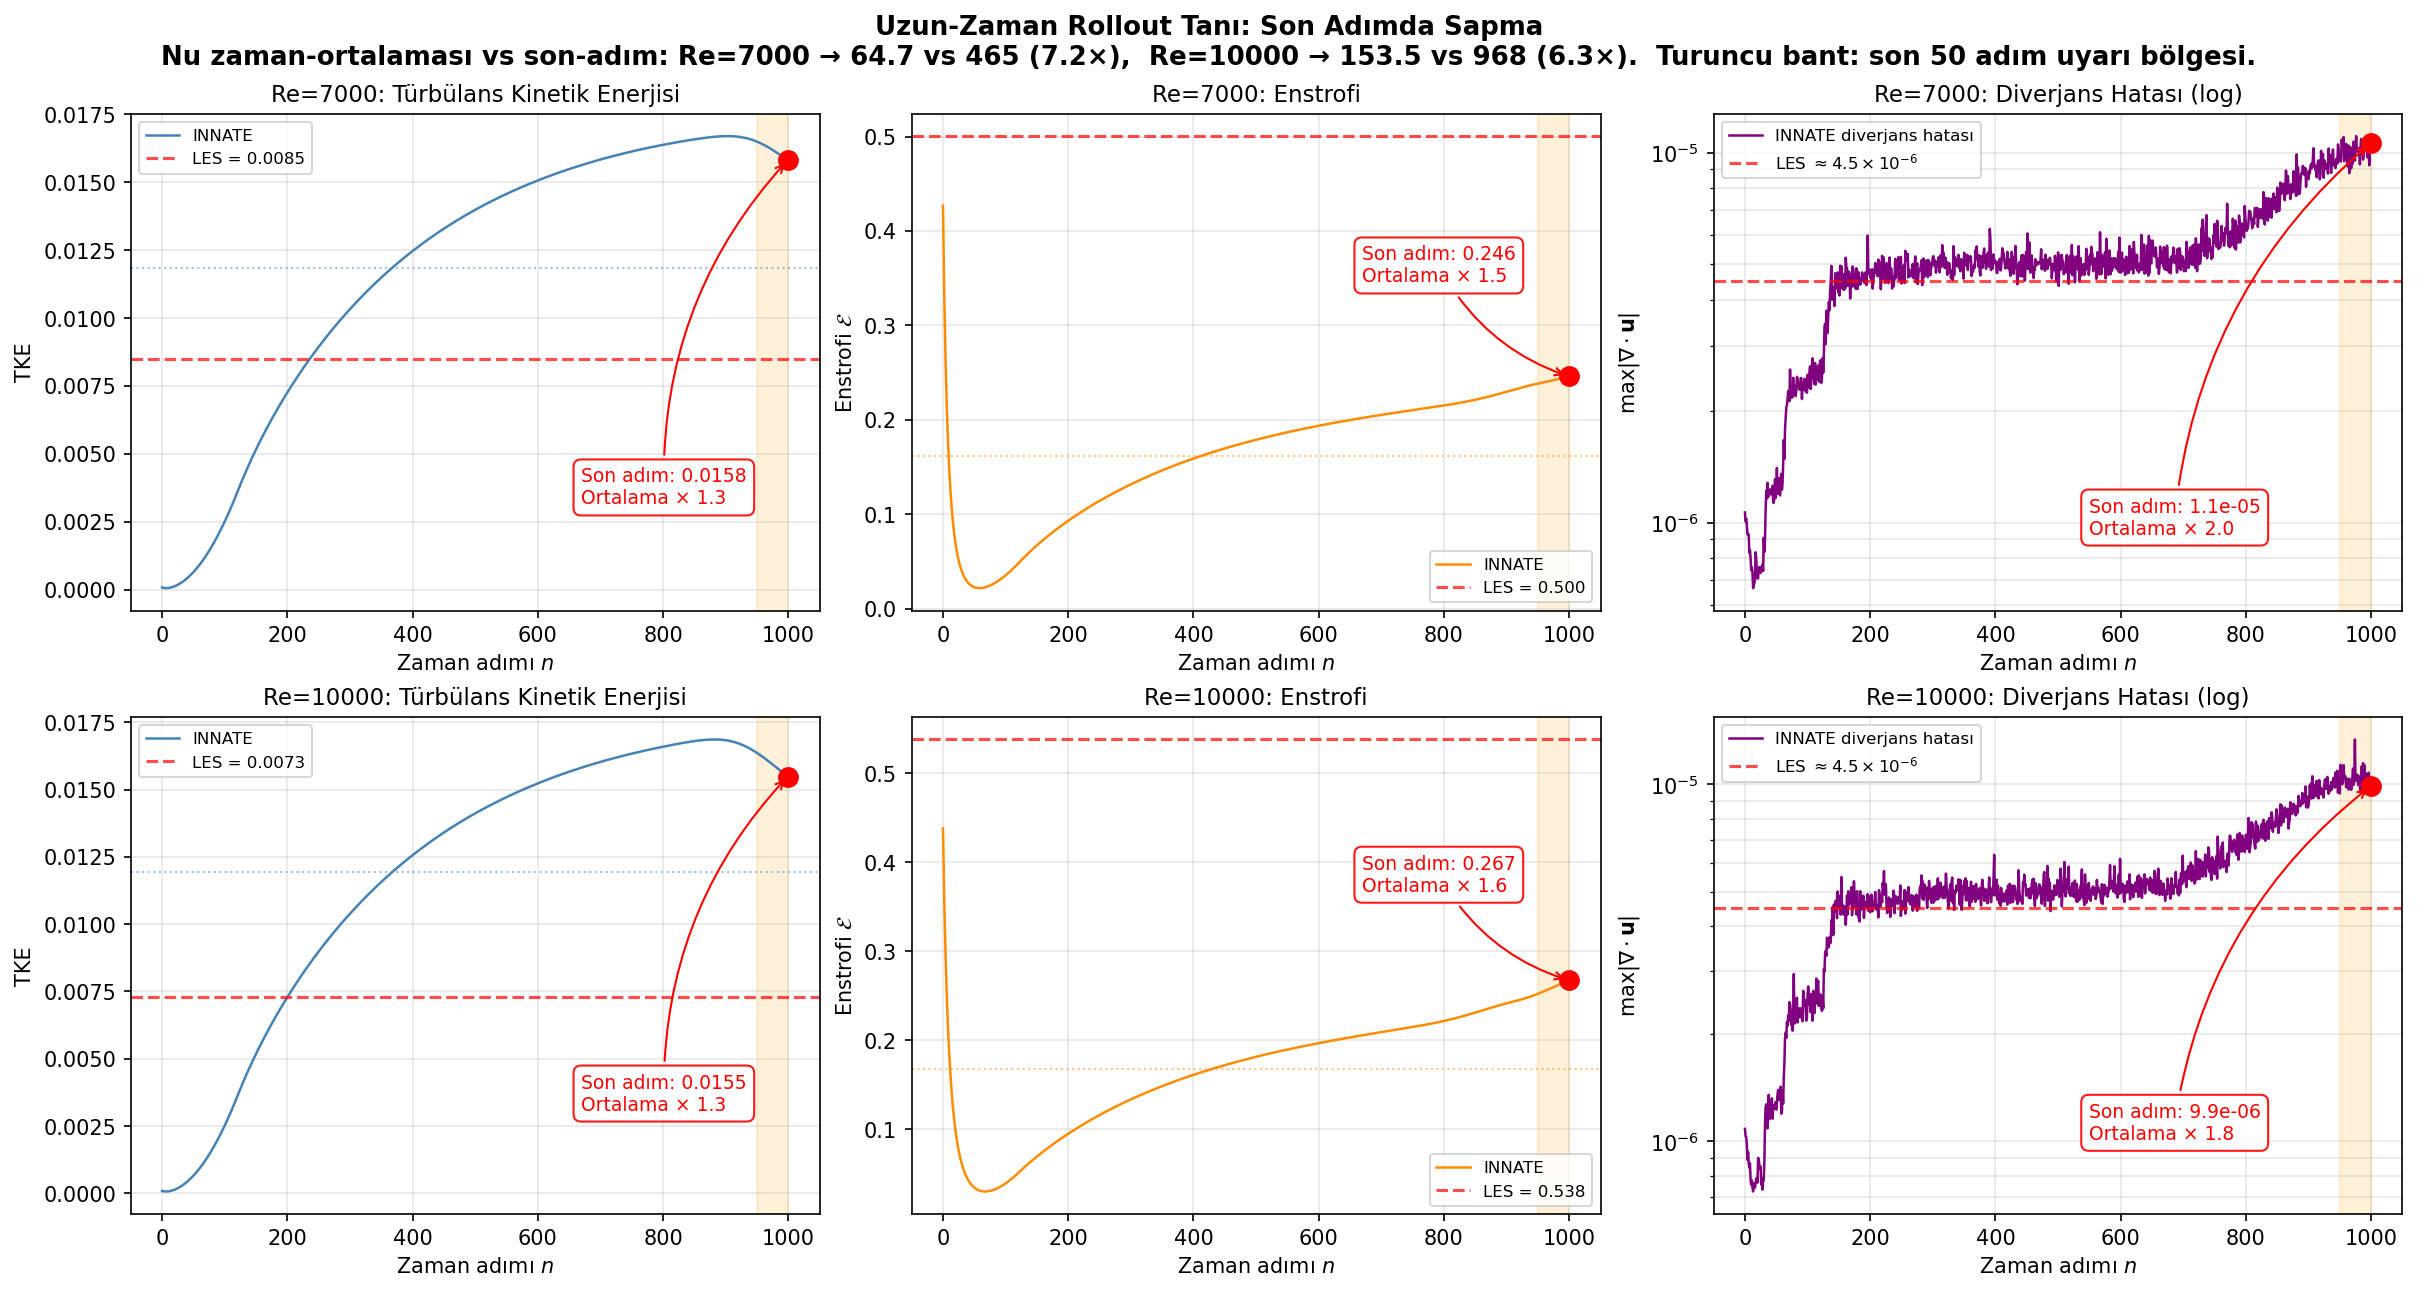
\includegraphics[width=17cm]{figurler/fig_09_son_adim_sicrama.png}}
\caption{Eğitilen INNATE modelinin uzun-zaman rollout'u boyunca temel niceliklerin zaman serileri (Re=7000 üst sıra, Re=10\,000 alt sıra). Soldan sağa: TKE (lineer ölçek), enstrofi (lineer ölçek), maksimum diverjans hatası (log ölçek). Kırmızı kesikli yatay çizgiler LES referans değerleridir; turuncu bant son 50 zaman adımındaki uyarı bölgesidir; kırmızı noktalar son adımdaki değerleri, kutular ise ortalamaya göre oranlarını göstermektedir.}
\label{fig:son_adim_sicrama}
\end{figure}

Üç temel gözlem ortaya çıkar.

\paragraph{Momentum nicelikleri orta düzey sapma gösterir.} TKE değerleri her iki Reynolds sayısında da ortalama değerin yaklaşık $1.3$ katına ulaşmıştır; enstrofi $1.5$--$1.6$ katına, maksimum diverjans hatası ise $1.8$--$2.0$ katına ulaşmıştır. Bu değerler, modelin son zaman adımlarında bir miktar nümerik gerilim biriktirdiğini göstermekle birlikte, mertebe büyüklüğü değiştiren bir kararsızlık değildir. Diverjans hatası logaritmik ölçekte gösterildiği için artış görsel olarak belirgindir; ancak mutlak değer ($\sim 10^{-5}$) LES referans seviyesinin ($\sim 5\times 10^{-6}$) yalnızca iki katı düzeyinde kalmıştır.

\paragraph{Nusselt sayısı anormal sıçrama gösterir.} Buna karşılık Nusselt sayısının zaman-ortalama ile son-adım değerleri arasındaki oran $6$--$7$ katına ulaşmaktadır. Bu oran momentum niceliklerindeki sıçrama oranından (en fazla $2\times$) çok daha büyüktür. Tek başına TKE veya enstrofideki sapma, ortalama hızın ya da vortisitenin ortalama yaklaşık $1.3$--$1.6$ katına çıkmasına karşılık gelir; bu Nu'da yalnızca $\mathcal{O}(\sqrt{1.3}\cdot 1.6)\approx 1.8$ kat artış doğurabilir. Dolayısıyla Nu'daki $6$--$7$ katlık sıçrama momentum kanalıyla açıklanamaz.

\paragraph{Sapmanın termal akı kanalında lokal kaldığı sonucu.} Bu gözlem, son-adım sıçramasının kök sebebinin $\langle v\theta\rangle$ konvektif ısı akısının anlık bir tepe değerine ulaşması olduğunu göstermektedir. Tekrar hatırlatmak gerekirse, Bölüm~\ref{sec:termal_sinir}'de termal alanın momentum alanına kıyasla daha zayıf modellendiği belirtilmişti; alt-ızgara difüzivitesi yalnızca tek skaler $\mathrm{Pr}_{t}^{(\ell)}$ parametresine bağlı, termal alanın spektral şekli için bir kayıp terimi mevcut değil. Bu yapısal zayıflıklar uzun-zaman rollout'unda toplam etki olarak termal akı kanalında anlık tepe değerlerine yol açmıştır.

\paragraph{Etki ve sonuç.} Bu tanı, modelin değerlendirme metriklerinde \emph{zaman-ortalamalı} Nusselt sayısının kullanılmasını gerektirir; tek-noktada raporlama (örneğin yalnızca son-adım Nu değeri) modelin gerçek istatistiksel davranışını yansıtmaz ve okuyucuyu yanıltır. Aynı zamanda bu bulgu, gelecek çalışmaların termal kanal modellemesini önceliklendirmesi gerektiğine somut bir kanıt sunar; momentum kanalının kararlılığını korurken termal alanın spektral kapanışını güçlendirecek mimari iyileştirmeler (örneğin termal Spectral-Cs parametrizasyonu, termal spektrum şekil kaybı) Bölüm~\ref{ch:sonuc}'de ele alınmıştır.

\subsection{Spectral-Cs Parametre Aktivasyonu}
\label{sec:spectral_cs_aktivasyon}

Eğitilen modelin Spectral-Cs parametrelerinin son değerleri incelendiğinde, Fourier katsayılarının ($a^{(\ell)}_{\mathbf{k}}$) büyük çoğunluğunun başlangıç değerlerinden anlamlı biçimde uzaklaşmadığı görülmüştür. Katman-başına baz Smagorinsky sabiti $C_{s,0}^{(\ell)}$ özellikle son üç katmanda (katman 18--20) anlamlı düşüş göstermiş ($\sim 0.173$'ten $\sim 0.138$'e), türbülans Prandtl sayısı $\mathrm{Pr}_{t}^{(\ell)}$ de bu katmanlarda hafif artmıştır ($0.834 \to 0.864$); ancak uzaysal değişim üreten Fourier katsayıları görece küçük kalmıştır.

Bu davranışın temel kaynağı, çalışmanın eğitim bütçesinin (RTX~4090 dizüstü GPU üzerinde 100 epoch, $\sim 6$ saat) sınırlı olmasıdır. Daha uzun eğitim süreleri (örneğin 500--1000 epoch) ve daha güçlü donanım altında, optimizer'in Fourier katsayılarını başlangıç değerlerinden uzaklaştırma yönünde yeterli gradyan akümülasyonu yapması ve böylece tam uzaysal kapasitenin aktive olması beklenmektedir. Bu çalışmanın kapsamında Spectral-Cs parametrizasyonu \emph{mimari kapasite} olarak sunulmuş, tam uzaysal aktivasyonun değerlendirilmesi gelecek çalışmalara bırakılmıştır.

\section{Zamansal Görselleştirme}
\label{sec:zamansal}

Modelin uzun-zaman dinamiklerini incelemek için merkezi $z$-dilim ($z=L_{z}/2$) üzerindeki hız büyüklüğü ve sıcaklık dalgalanması alanlarının dört farklı zaman noktasındaki görüntüleri Şekil~\ref{fig:slice_4zaman}'de sunulmuştur. Bu görüntüler, modelin büyük-ölçek yapıları (Kolmogorov forcing'in dört karşıt-dönen hücresi) kararlı biçimde koruduğunu, ancak küçük ölçekli detayların LES'e kıyasla daha düzgün (daha yumuşatılmış) olduğunu nitel olarak doğrular.

\begin{figure}[H]
\centering
\makebox[\textwidth][c]{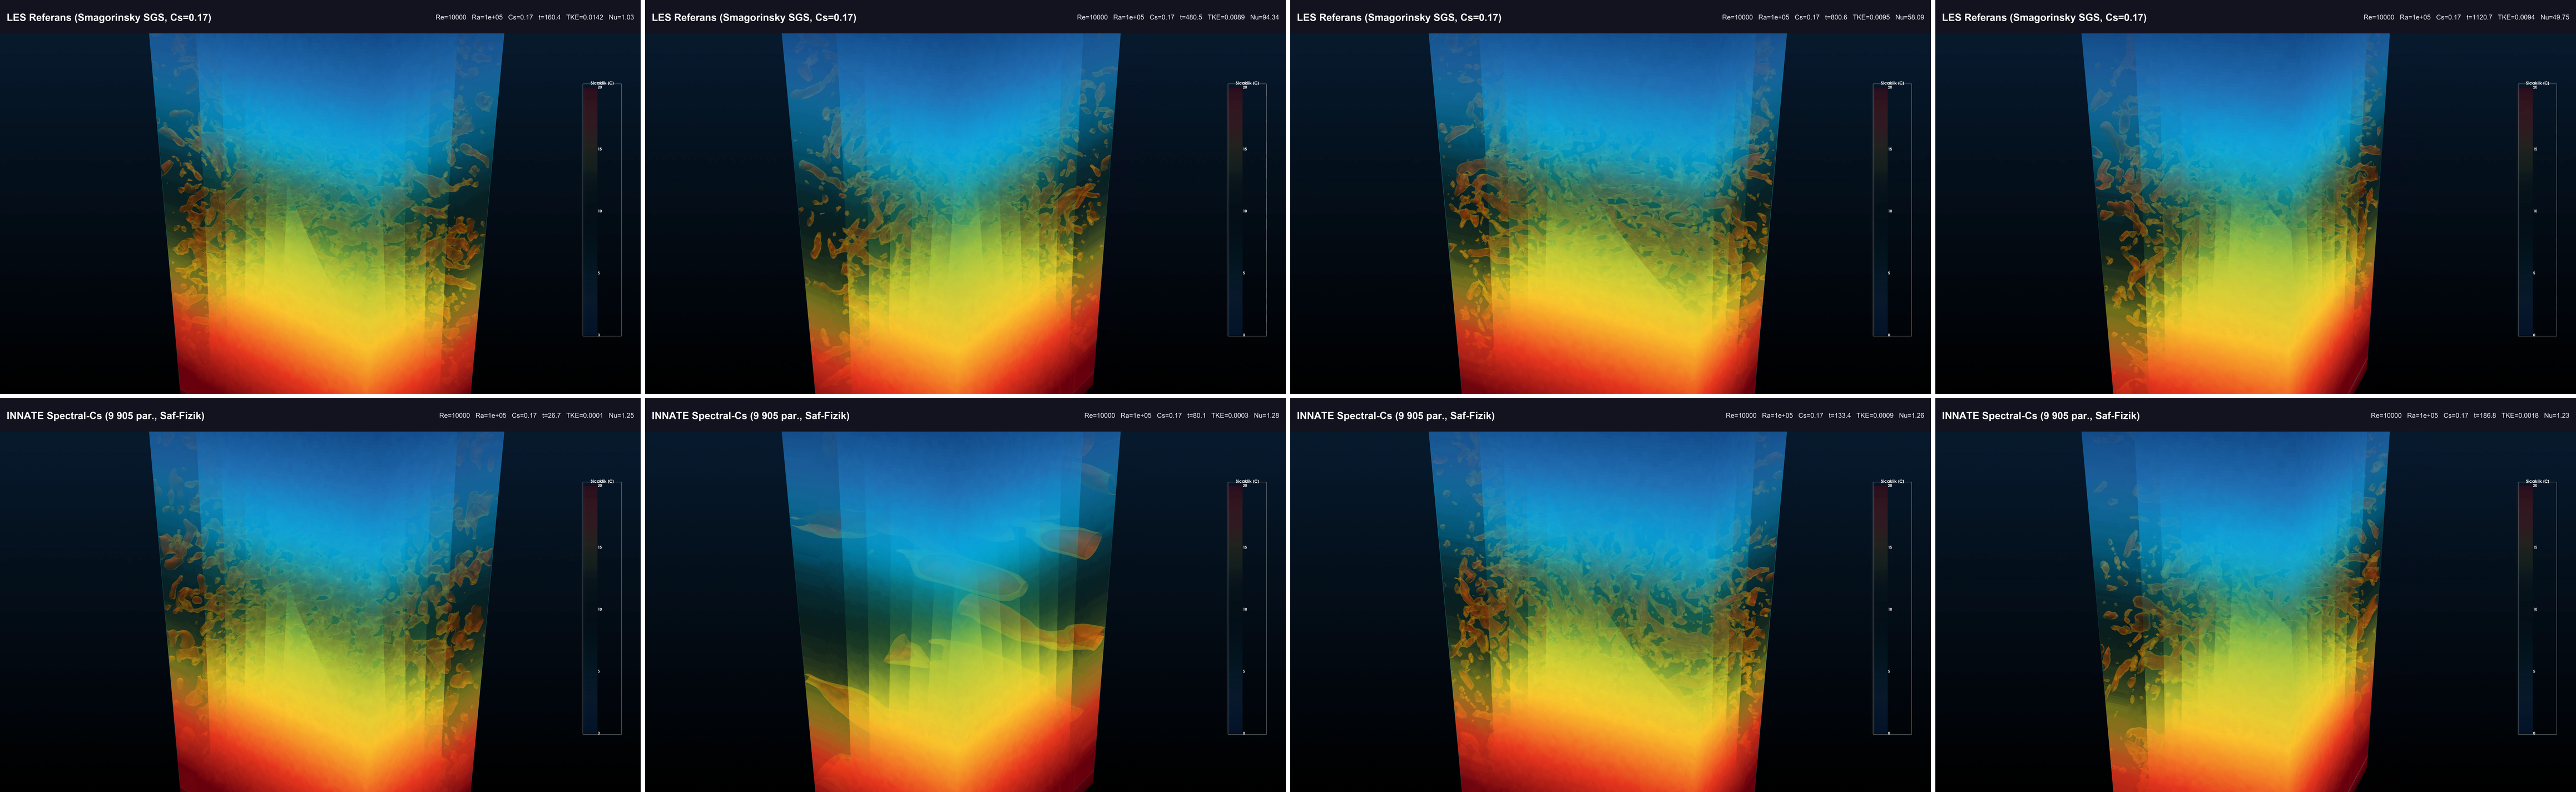
\includegraphics[width=17cm]{figurler/fig_11_slice_4zaman_clean.png}}
\caption{Sıcaklık alanının 3B hacim görselleştirmesi, dört farklı zaman noktasında (soldan sağa, eğitim mesafesinin $\sim$$\tfrac{1}{4}, \tfrac{1}{2}, \tfrac{3}{4}$ ve sonu). Üst sıra: LES referans (Smagorinsky $C_{s}=0.17$). Alt sıra: INNATE Spectral-Cs 9905 parametre. Renk skalası: sıcak (kırmızı, alt) -- ılık (sarı) -- soğuk (mavi, üst); her panelin sağında bağımsız colorbar mevcuttur. Görüntüler tez ekindeki 4K videolardan (\texttt{les\_3d\_4k\_30s.mp4}, \texttt{innate\_3d\_4k\_30s.mp4}) eşit zaman aralıklarında alınmıştır. Modelin büyük-ölçek termal pleym yapısını (alt sıcak akışkan yukarı taşınımı) doğru yöne öğrendiği ancak küçük-ölçek karışım detaylarını LES'e kıyasla daha yumuşatılmış üretmesi nitel olarak görülmektedir.}
\label{fig:slice_4zaman}
\end{figure}

INNATE modelinin LES referansı ile yan yana 3D görselleştirme videoları (\texttt{innate\_3d\_4k\_30s.mp4}, \texttt{les\_3d\_4k\_30s.mp4}) tez ekinde sunulmuş olup sözlü sunum sırasında ekran üzerinde gösterilecektir; bu videolar, tezde statik figürler aracılığıyla aktarılamayan akış-yapısı dinamiğini görsel olarak doğrular.

Eval karşılaştırmasının özet bir paneli Şekil~\ref{fig:eval_karsilastirma}'da sunulmuş ve tüm temel metriklerin tek bir bakışta değerlendirilmesi sağlanmıştır.

\begin{figure}[H]
\centering
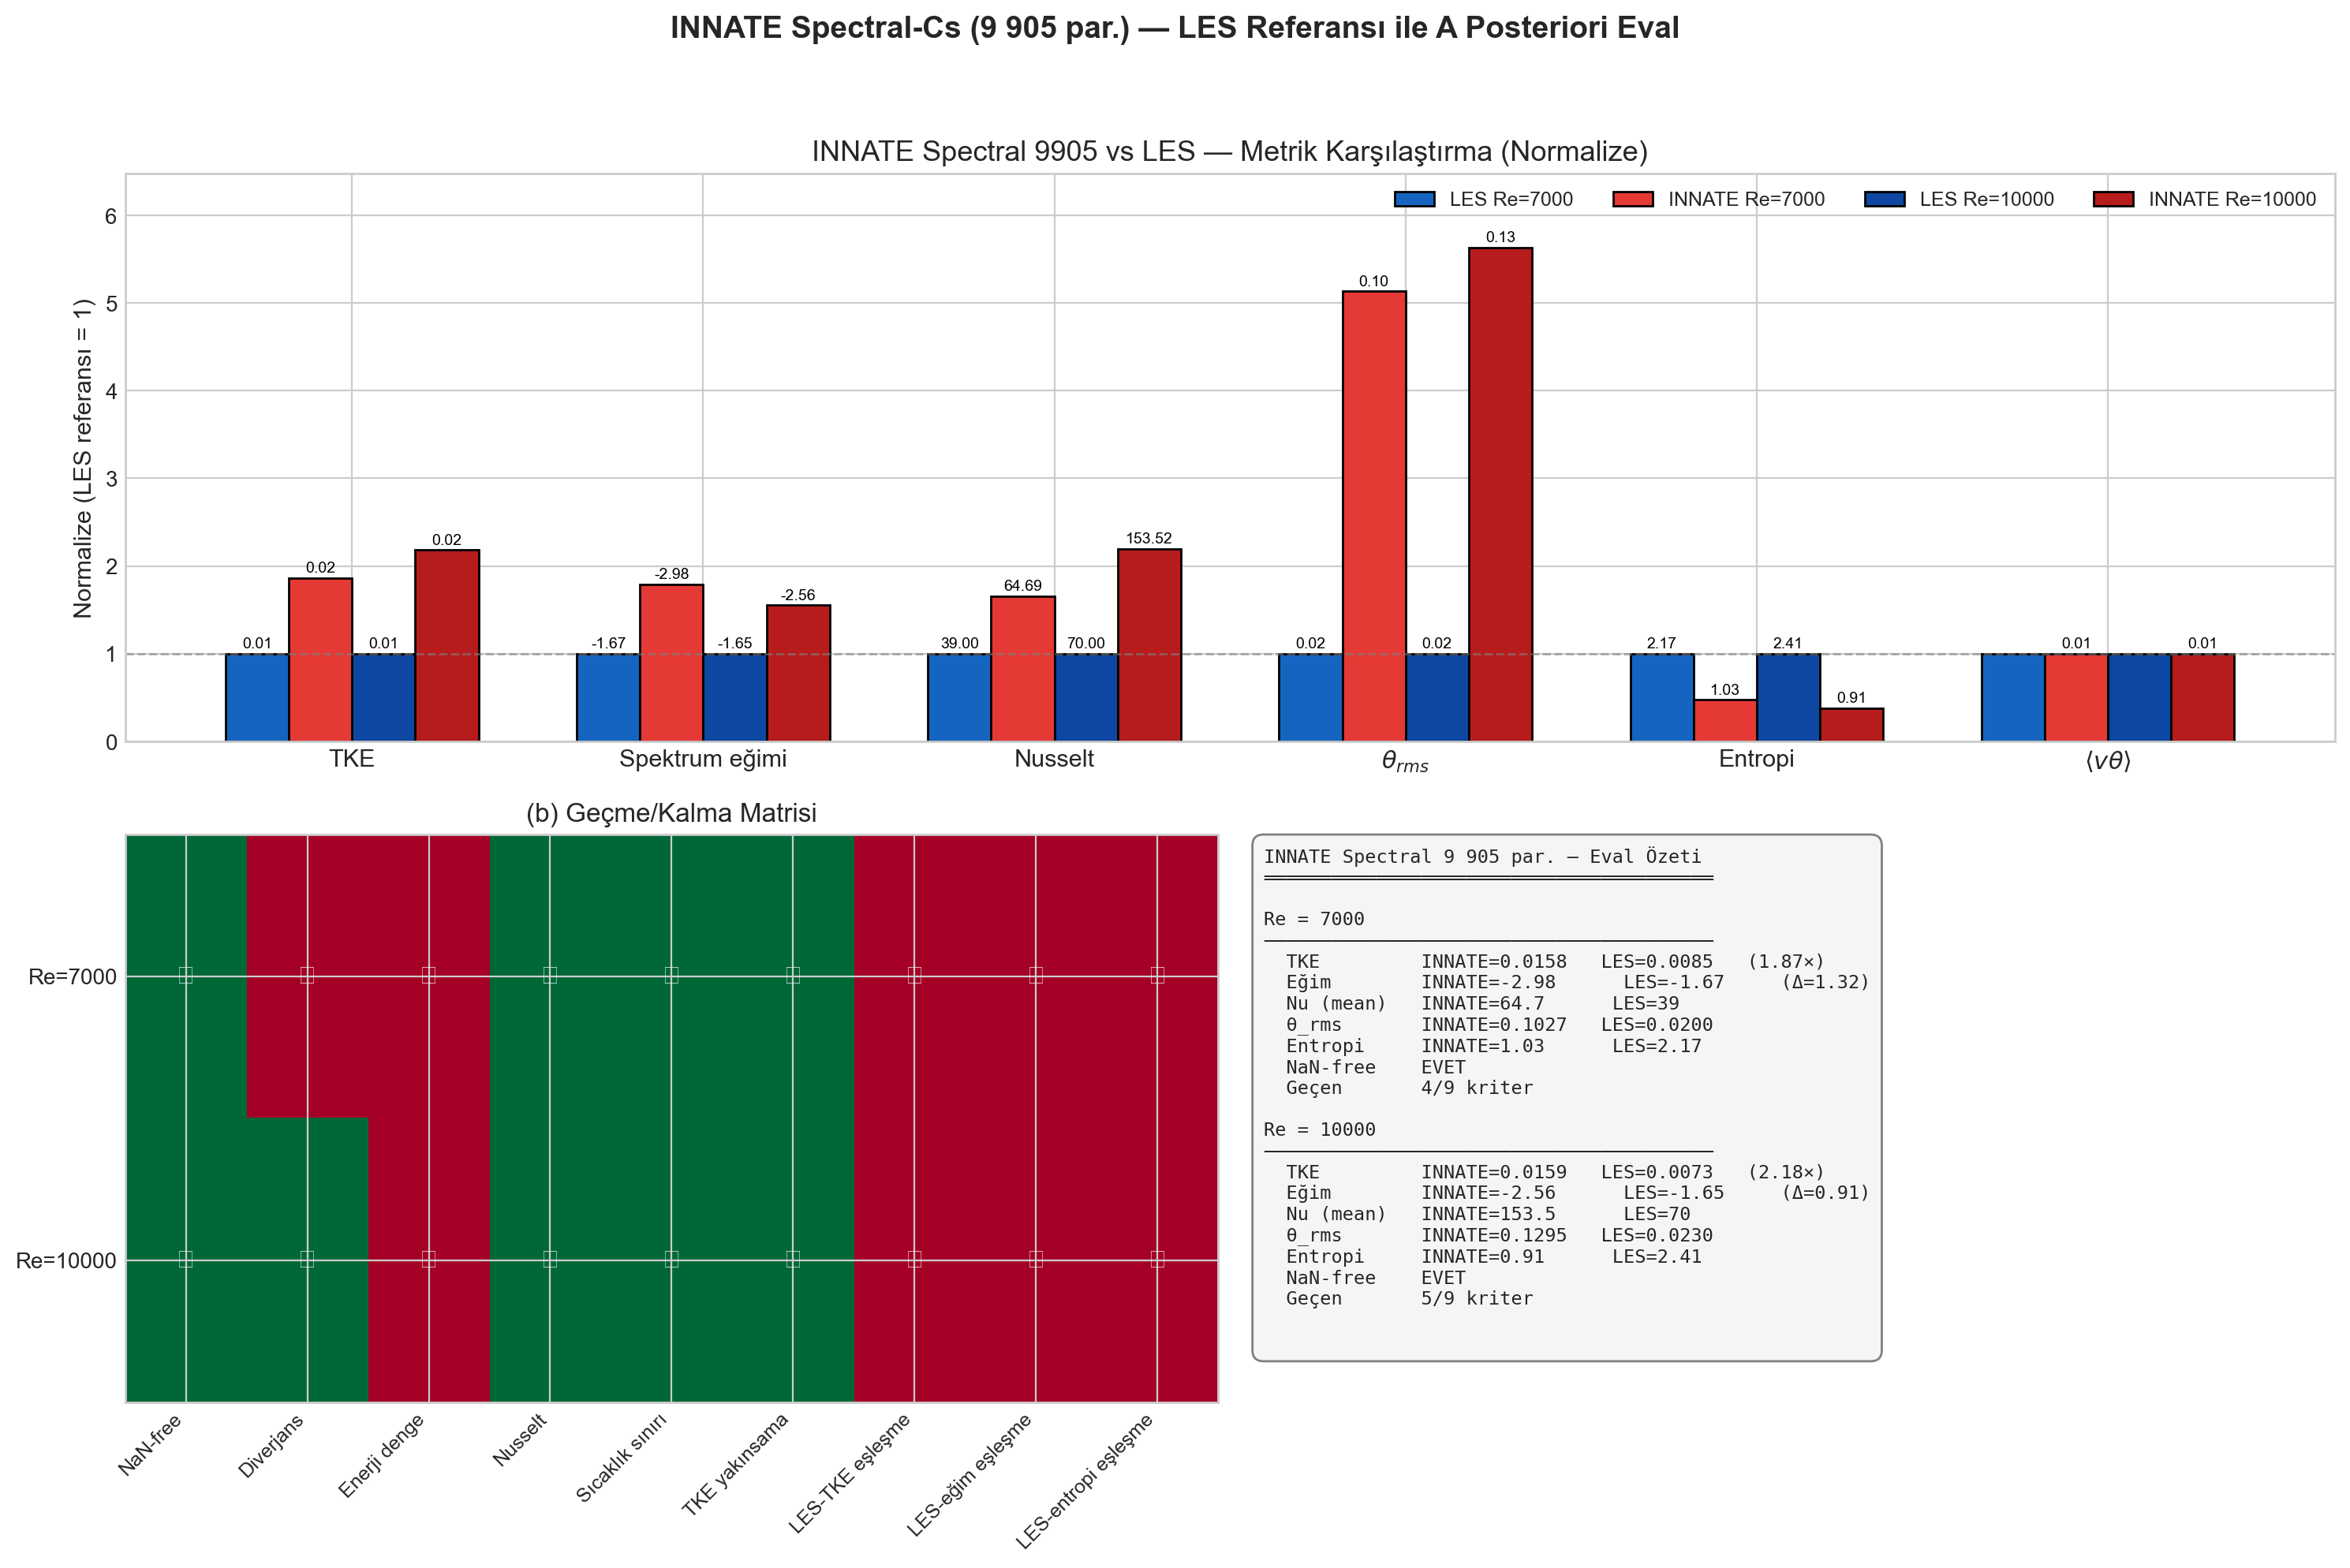
\includegraphics[width=15.5cm]{figurler/fig_04_eval_karsilastirma.png}
\caption{INNATE modeli ile LES referansı arasındaki kapsamlı eval karşılaştırma paneli.}
\label{fig:eval_karsilastirma}
\end{figure}
